% 注释的快捷键: Ctrl + /

% \documentclass[a4paper]{ctexart}
\documentclass{book}

\usepackage{xeCJK}
\usepackage{amsmath, amssymb, amsfonts, amsthm}
\usepackage{mathrsfs}
\usepackage{gensymb}
\usepackage{graphicx}
\usepackage{hyperref}
\usepackage{url}
\usepackage{cases}
\usepackage{color}
\usepackage{tikz-cd}
% \usepackage{times}
% \usepackage{mathptmx}
% \DeclareMathAlphabet{\mathcal}{OMS}{cmsy}{m}{n}
% \DeclareSymbolFont{largesymbols}{OMX}{cmex}{m}{n}

% \usepackage{unicode-math}
% \setmathfont{XITS Math}
% \setmathfont{XITS Math}[StylisticSet=1,range=cal]

%下面是引用前文定理的代码
% \usepackage{hyperref}
% \begin{lemma}[test]\label{test}
	%     test
	%   \end{lemma}

%   number: \ref{test}, name: \nameref{test}

%如何在等号上加文字或记号
%通过 \stackrel{?}{=}

% 如何实现大括号多编号
% \usepackage{cases}
% \begin{numcases}{}
% 	x_1&=eq1 \label{eqsystem1} \\
% 	x_2+1&=eq2 \label{eqsystem2}
% \end{numcases}

% 如何插入交换图


\newtheorem{theorem}{\indent 定理}[section]
\newtheorem{definition}[theorem]{\indent 定义}
\newtheorem{proposition}[theorem]{\indent 命题}
\newtheorem{lemma}[theorem]{\indent 引理}
\newtheorem{corollary}[theorem]{\indent 推论}
\newtheorem{example}[theorem]{\indent 例}
\newtheorem{problem}[theorem]{\indent 问题}
\newtheorem*{remark}{\indent 注}
\renewcommand{\proofname}{\indent \bf 证明}
\newcommand{\pd}[2]{\frac{\partial #1}{\partial #2}} %一次偏导
\newcommand{\npd}[3]{\frac{\partial^{#1}{#2}}{\partial{#3}^{#1}}} %n次偏导, 也可以指代混合偏导
\newcommand{\pD}[2]{\frac{{\rm D}(#1)}{{\rm D}(#2)}} %Jacobian
\newcommand{\lc}[2]{\nabla_{#1}{#2}}
\newcommand{\ft}[3]{{#1}_{#2},\dots,{#1}_{#3}}
\newcommand{\cft}[3]{{#1}_{#2},\cdots,{#1}_{#3}}
\newcommand{\id}{{\rm id}}
\newcommand{\supp}{{\rm supp}}
\newcommand{\mi}{\sqrt{-1}}
\newcommand{\me}{{\rm e}}
\newcommand{\md}{{\rm d}}
\newcommand{\mZ}{\mathbb{Z}}
\newcommand{\mQ}{\mathbb{Q}}
\newcommand{\mR}{\mathbb{R}}
\newcommand{\mC}{\mathbb{C}}
\newcommand{\GL}{{\rm GL}}
\newcommand{\SL}{{\rm SL}}
\newcommand{\Aut}{{\rm Aut}}
\newcommand{\Inn}{{\rm Inn}}
\newcommand{\Lie}{{\rm Lie}}


% \graphicspath{{Figures/}}

\allowdisplaybreaks

\begin{document}

    \title{数学笔记}
    \author{BeBop}
    \maketitle
    \newpage

    \tableofcontents
    \newpage
    
    \part{知识整理}
    % \chapter{高等代数}
\section{线性空间、对偶空间}
    \subsection{对偶空间}

    \subsection{协变张量与反变张量}

    “The general formulation of covariance and contravariance refers to 
    how the components of a coordinate vector transform under a change of basis.”
    协变张量与反变张量描述了向量的坐标分量是如何随基向量的变化而变化的.

    设线性空间 $V$ 有两组基:
    \begin{align*}
        &\{e_i\}:\quad e_1,\dots,e_n \\
        &\{{e}'_i\}:\quad {e'}_1,\dots,{e'}_n
    \end{align*}
    它们的对偶基分别为
    \begin{align*}
        &\{{e^*}_i\}:\quad {e^*}_1,\dots,{e*}_n \\
        &\{{e^*}'_i\}:\quad {e^*}'_1,\dots,{e^*}'_n
    \end{align*}
    并且 $\{e_i\}$ 到 $\{{e}'_i\}$ 的过渡矩阵为 $P = (a_{ij})$, 即
    \begin{equation*}
        ({e'}_1,\dots,{e'}_n) = (e_1,\dots,e_n)P = (e_1,\dots,e_n)
        \begin{pmatrix}
            a_{11} & \cdots & a_{1n} \\
            \vdots & & \vdots \\
            a_{n1} & \cdots & a_{nn}
        \end{pmatrix}
    \end{equation*}

    \textbf{反变张量: }设 $v$ 是 $V$ 中的某个向量, 它在基 $\{e_i\},\,\{{e'}_i\}$ 下的坐标 $v[e_i],\,v[{e'}_i]$ 分别为 $\{X_i\}$ 和 $\{{X'}_i\}$, 即
    \begin{equation*}
        v = 
        \begin{pmatrix}
            e_1,\dots,e_n
        \end{pmatrix}
        \begin{pmatrix}
            x_1 \\ \vdots \\ x_n
        \end{pmatrix} = 
        \begin{pmatrix}
            {e'}_1,\dots,{e'}_n
        \end{pmatrix}
        \begin{pmatrix}
            {x'}_1 \\ \vdots \\ {x'}_n
        \end{pmatrix}
    \end{equation*}
    则由
    \begin{equation*}
        v = 
        \begin{pmatrix}
            {e'}_1,\dots,{e'}_n
        \end{pmatrix}
        \begin{pmatrix}
            {x'}_1 \\ \vdots \\ {x'}_n
        \end{pmatrix} = 
        \begin{pmatrix}
            e_1,\dots,e_n
        \end{pmatrix}
        P
        % \begin{pmatrix}
        %     a_{11} & \cdots & a_{1n} \\
        %     \vdots & & \vdots \\
        %     a_{n1} & \cdots & a_{nn}
        % \end{pmatrix}
        \begin{pmatrix}
            {x'}_1 \\ \vdots \\ {x'}_n
        \end{pmatrix}
    \end{equation*}
    知
    \begin{equation*}
        \begin{pmatrix}
            x_1 \\ \vdots \\ x_n
        \end{pmatrix} = 
        P
        % \begin{pmatrix}
        %     a_{11} & \cdots & a_{1n} \\
        %     \vdots & & \vdots \\
        %     a_{n1} & \cdots & a_{nn}
        % \end{pmatrix}
        \begin{pmatrix}
            {x'}_1 \\ \vdots \\ {x'}_n
        \end{pmatrix}
    \end{equation*}
    于是
    \begin{equation*}
        \begin{pmatrix}
            {x'}_1 \\ \vdots \\ {x'}_n
        \end{pmatrix} = 
        P^{-1}
        % \begin{pmatrix}
        %     a_{11} & \cdots & a_{1n} \\
        %     \vdots & & \vdots \\
        %     a_{n1} & \cdots & a_{nn}
        % \end{pmatrix}^{-1}
        \begin{pmatrix}
            x_1 \\ \vdots \\ x_n
        \end{pmatrix}
    \end{equation*}
    从表达式可以看出 $v$ 坐标分量的变化与基向量的变化是相反的, 也可以这么理解: $v$ 本就是不随基底改变的一个固有对象, 为了保持不变, 
    它坐标分量的变化必须与基底变化相反, 才能抵消基变换带来的影响, 用式子表示即为
    \begin{align*}
        v &= 
        \begin{pmatrix}
            e_1,\dots,e_n
        \end{pmatrix}
        \begin{pmatrix}
            x_1 \\ \vdots \\ x_n
        \end{pmatrix} \\ &= 
        \begin{pmatrix}
            e_1,\dots,e_n
        \end{pmatrix}PP^{-1}
        \begin{pmatrix}
            x_1 \\ \vdots \\ x_n
        \end{pmatrix} \\ &= 
        \begin{pmatrix}
            {e'}_1,\dots,{e'}_n
        \end{pmatrix}
        \begin{pmatrix}
            {x'}_1 \\ \vdots \\ {x'}_n
        \end{pmatrix}
    \end{align*}

    \textbf{共变张量:}设 $f$ 是对偶空间 $V^*$ 中的元素, 即 $f$ 是 $V$ 上的线性函数, $\{y_i\} = \{f[e_i]\},\,\{{y'}_i\} = \{f[{e'}_i]\}$ 为它在这两组基下的坐标, 即
    \begin{align*}
        f &= \sum_{i=1}^{n}y_i e^*_i = \sum_{i=1}^{n}f(e_i)e^*_i \\
        &= \sum_{i=1}^{n}y'_i {e^*}'_i = \sum_{i=1}^{n}f(e'_i){e^*}'_i
    \end{align*}
    而
    \begin{align*}
        \begin{pmatrix}
            y'_1, \dots, y'_n
        \end{pmatrix} &= 
        \begin{pmatrix}
            f(e'_1), \dots, f(e'_n)
        \end{pmatrix} \\
        &= f\left(
            \begin{pmatrix}
                {e'}_1,\dots,{e'}_n
            \end{pmatrix}
        \right) \\
        &= f\left(
            \begin{pmatrix}
                e_1,\dots,e_n
            \end{pmatrix} P
        \right) \\
        &= \begin{pmatrix}
            f(e_1), \dots, f(e_n)
        \end{pmatrix}P \\
        &= \begin{pmatrix}
            y_1, \dots, y_n
        \end{pmatrix}P
    \end{align*}
    所以 $f$ 的坐标的变化与基底的变化保持一致.

\section{线性映射、线性变换的矩阵表示}

    设线性映射 $\mathcal{A}:V\rightarrow W$, $(\xi^1,\xi^2,\dots,\xi^m)$ 是 $V$ 的一组基, $(\eta^1,\eta^2,\dots,\eta^n)$ 是 $W$ 的一组基, 那么 $\mathcal{A}$ 在这两组基下的矩阵为,
    \begin{equation*}
        \mathcal{A}(\xi^1,\dots,\xi^m)=(\mathcal{A}\xi^1,\dots,\mathcal{A}\xi^m)=(\eta^1,\dots,\eta^n)
        \begin{pmatrix}
            a_{11} & \cdots & a_{1m} \\
            \vdots &        & \vdots \\
            a_{n1} & \cdots & a_{nm}
        \end{pmatrix} = (\eta^1,\dots,\eta^n)A
    \end{equation*}

    设 $v$ 是 $V$ 中的向量, 并设
    \begin{equation*}
        v=x_1\xi^1+\cdots+x_m\xi^m=(\xi^1,\dots,\xi^m)
        \begin{pmatrix}
            x_1 \\
            \vdots \\
            x_m
        \end{pmatrix}=(\xi^1,\dots,\xi^m)X
    \end{equation*}
    其中 $X$ 是 $v$ 在基 $(\xi^1,\dots,\xi^m)$ 下的坐标, 那么由于
    \begin{align*}
        \mathcal{A}v &=\mathcal{A}(x_1\xi^1+\cdots+x_m\xi^m) \\
        &=\mathcal{A}(\xi^1,\dots,\xi^m)
        \begin{pmatrix}
            x_1 \\
            \vdots \\
            x_m
        \end{pmatrix} \\
        &=(\mathcal{A}\xi^1,\dots,\mathcal{A}\xi^m)
        \begin{pmatrix}
            x_1 \\
            \vdots \\
            x_m
        \end{pmatrix} \\
        & = (\eta^1,\dots,\eta^n)
        \begin{pmatrix}
            a_{11} & \cdots & a_{1m} \\
            \vdots &        & \vdots \\
            a_{n1} & \cdots & a_{nm}
        \end{pmatrix}
        \begin{pmatrix}
            x_1 \\
            \vdots \\
            x_m
        \end{pmatrix} \\
        & = (\eta^1,\dots,\eta^n)AX
    \end{align*}
    $\mathcal{A}v$ 在基 $(\eta^1,\eta^2,\dots,\eta^n)$ 下的坐标为 $AX$.

\section{矩阵迹的几何解释}
    给定一个矩阵 $A = (a_{ij})_{n\times n}$, 在高代中我们定义了矩阵的迹为:
    \begin{equation*}
        {\rm tr}(A) = \sum_{i = 1}^{n}a_{ii}
    \end{equation*}
    下面我们从比较几何的角度给出矩阵迹的一个定义, 并用这个定义重新证明关于迹的一些性质.

\subsection{用矩阵定义的向量场}
    设矩阵  $A$ 如上, 定义 $\mathbb{R}^n$ 上的向量场 $F_A(X) := AX,\,\forall X\in\mathbb{R}^n$.
    则可证明向量场 $F_A$ 的散度 ${\rm div}(F_A)$ 是常数, 且经计算恰好是我们所熟知的 $A$ 的迹, 我们就把这个值作为矩阵迹的定义, 即
    \begin{equation*}
        {\rm div}F_A := {\rm tr}A
    \end{equation*}
    \begin{remark}
        矩阵 $A$ 对应某个线性变换 $\mathcal{A}\in\mathrm{End}(\mathbb{R}^n)$, 从函数角度来看,   $X\mapsto AX$ 是一个从 $\mathbb{R}^n$ 到 $\mathbb{R}^n$ 的向量值函数.
        因为每个 $\mathbb{R}^n$ 上的函数都可视作 $\mathbb{R}^n$ 的向量丛的截面, 也即 $\mathbb{R}^n$ 上的光滑向量场, 这也解释了为什么这么定义 $F_A$.
    \end{remark}
    \begin{remark}
        我们可以从多变量微积分的角度验证新定义的合理性,
        \begin{equation*}
            F_A(x^1,\dots,x^n) = (\sum_{i=1}^{n}a_{1i}x^i,\dots,\sum_{i=1}^{n}a_{ni}x^i).
        \end{equation*}
        则
        \begin{equation*}
            (\mathrm{div} F_A)(p) = \sum_{i=1}^{n}\frac{\partial F_A^i}{\partial x^i}\Bigg|_p = \sum_{i=1}^{n}a_{ii}
        \end{equation*}
        结果是一个常数且取值就是我们熟知的迹.
    \end{remark}
    因为上述求散度计算中仍有取主对角线元素相加的操作, 形式上和最原始的定义没有本质区别, 所以下面用微分形式的语言重新计算散度.

    取 $\mathbb{R}^n$ 中的平坦度量, 并取自然坐标系 $(x^1,\dots,x^n)$, 则体积形式为
    \begin{equation*}
        \Omega = \md x^1\wedge\cdots\wedge\md x^n
    \end{equation*}
    向量场 $F_A$ 的表达式为
    \begin{equation*}
        F_A(x^1,\dots,x^n) = \sum_{i,\,j}a_{ij}x^j\frac{\partial}{\partial x^i}\Bigg|_{(x^1,\dots,x^n)}
    \end{equation*}
    向量场 $F_A$ 的散度定义为
    \begin{equation}\label{div}
        (\mathrm{div}F_A)\Omega = L_{F_A}\Omega
    \end{equation}
    因为
    \begin{equation*}
        L_{F_A}\md x^i = \md L_{F_A}x^i
        = \md (F_Ax^i)
        = \md \sum_{k=1}^{n}a_{ik}x^k
        = \sum_{k=1}^{n}a_{ik}\md x^k
    \end{equation*}
    所以
    \begin{align*}
        L_{F_A}\Omega &= L_{F_A}(\md x^1\wedge\cdots\wedge\md x^n) \\
        &= \sum_{i=1}^{n}\md x^1\wedge\cdots\wedge L_{F_A}\md x^i \wedge\cdots\wedge\md x^n \\
        &= \sum_{i=1}^{n}\md x^1\wedge\cdots\wedge\left(\sum_{k=1}^{n}a_{ik}\md x^k\right)\wedge\cdots\wedge\md x^n \\
        &= \left(\sum_{i=1}^{n}a_{ii}\right)\md x^1\wedge\cdots\wedge\md x^n \\
        &= \left(\sum_{i=1}^{n}a_{ii}\right)\Omega
    \end{align*}
    经过一通计算我们再次验证了这么定义矩阵迹的合理性, 更进一步地, 我们可以用外微分的语言重新证明迹的几个性质, 比如, $\mathrm{tr}AB = \mathrm{tr}BA$.
    
    \subsection{迹的性质}
    我们知道关于李导数和李括号有等式
    \begin{equation*}
        [L_X, L_Y] = L_{[X,Y]}, \quad\forall X,\,Y\in C^{\infty}(\mathbb{R}^n,T\mathbb{R}^n)
    \end{equation*}
    设矩阵 $A = (a_{ij}),\,B = (b_{ij})$, 对应的向量场为 $F_A,\,F_B$, 因为
    \begin{equation*}
        \mathrm{ent}_{ij}[A,B] = \sum_{k=1}^{n}a_{ik}b_{kj}-b_{ik}a_{kj}
    \end{equation*}
    所以
    \begin{align*}
        [F_A,F_B] &= \sum_{i=1}^{n}\left(\sum_{j=1}^{n}F_A^j\frac{\partial F_B^i}{\partial x^j}-F_B^j\frac{\partial F_A^i}{\partial x^j}\right)\frac{\partial}{\partial x^i} \\
        &= \sum_{i=1}^{n}\left(\sum_{j=1}^{n}\sum_{k=1}^{n}a_{jk}b_{ij}x^k-b_{jk}a_{ij}x^k\right)\frac{\partial}{\partial x^i} \\
        &= \sum_{i=1}^{n}\left(\sum_{k=1}^{n}\left(\sum_{j=1}^{n}b_{ij}a_{jk}-a_{ij}b_{jk}\right)x^k\right)\frac{\partial}{\partial x^i} \\
        &= \sum_{i=1}^{n}\left(\sum_{k=1}^{n}\mathrm{ent}_{ik}[B,A]x^k\right)\frac{\partial}{\partial x^i} \\
        &= F_{[B,A]}
    \end{align*}
    因此
    \begin{align*}
        \mathrm{div}(F_{[B,A]})\Omega &= L_{F_{[B,A]}}\Omega \\
        &= L_{[F_A,F_B]}\Omega \\
        &= [L_{F_A},L_{F_B}]\Omega \\
        &= (L_{F_A}L_{F_B}-L_{F_B}L_{F_A})\Omega \\
        &= (\mathrm{div}F_A)(\mathrm{div}F_B)\Omega - (\mathrm{div}F_B)(\mathrm{div}F_A)\Omega \\
        &= 0
    \end{align*}
    从而推出
    \begin{equation*}
        \mathrm{tr}(BA-AB) = \mathrm{tr}[B,A] = \mathrm{div}F_{[B,A]} = 0
    \end{equation*}
    也即
    \begin{equation*}
        \mathrm{tr}(AB) = \mathrm{tr}(BA)
    \end{equation*}
    若 $A,\,B$ 不是 $n$ 阶方阵, 不妨设 $A = (a_{ij})_{m\times n},\,B = (b_{ij})_{n\times m}$, 其中 $m<n$,
    令 $A_1 = \begin{pmatrix}
        A_{m\times n} \\ O_{(n-m)\times n}
    \end{pmatrix},\,B_1 = \begin{pmatrix}
        B_{n\times m},\,O_{n\times(n-m)}
    \end{pmatrix}$
    于是有
    \begin{equation*}
        \mathrm{tr}(AB) = \mathrm{tr}(A_1B_1) = \mathrm{tr}(B_1A_1) = \mathrm{tr}(BA)
    \end{equation*}

\section{外代数与Lie代数}
    设 $V$ 是 $n$ 维线性空间, 我们有 $V$ 对应的外代数 $(E(V),\,\wedge)$, 也即
    \begin{equation*}
        E(V) = \bigoplus_{k=1}^{n}\bigwedge^{k}V
    \end{equation*}
    在 $E(V)$ 中我们可以定义 “微分” $\md$, 它满足:
    \begin{itemize}
        \item $\md\in{\rm End}(\bigwedge^{k}V,\,\bigwedge^{k+1}V),\quad k=0,\,1,\dots,\,n-1.$
        \item $\md(u_1\wedge\cdots\wedge u_s) = \sum\limits_{i = 1}^{s}(-1)^{i-1}u_1\wedge\cdots\wedge \md u_i\wedge\cdots\wedge u_s.$
        \item $\md\md u = 0\quad \forall u\in V.$
    \end{itemize}
    实际上我们只需定义线性映射
    \begin{align*}
        \md:V&\rightarrow\bigwedge^2V\\
        v&\mapsto\md v
    \end{align*}
    使其满足
    \begin{itemize}
        \item $\md(u\wedge v) = \md u\wedge v-u\wedge\md v$
    \end{itemize}
    再用线性性和外积使其扩充为 $E(V)$ 到自身的线性映射, 这样再加上 $\md^2 = 0$ 就可以定义一个微分运算了.

    接着上面的讨论, 我们考虑线性空间的对偶:
    \begin{align*}
        \md^*:\bigwedge^2V^*&\rightarrow V^*\\
        u\wedge v&\mapsto \md(u\wedge v)=:[u,v]
    \end{align*}
    我们有意把 $\md(u\wedge v)$ 记为 $[u,v]$ 是有考量的, 因为我们有如下定理:
    \begin{theorem}\label{lie}
        $\md$ 满足 $\md^2 = 0$ 当且仅当 $\md^*$ 满足 {\rm Jacobi} 恒等式, 此时 $(\mathfrak{g} = V,\,[\cdot,\cdot])$ 构成一个 {\rm Lie} 代数
    \end{theorem}
    \begin{proof}
        对 $\forall u\in V$, 设 
        \begin{align*}
            &\md u=\sum\limits_{i=1}^{r}v_i\wedge w_i \\
            &\md v_i=\sum\limits_{j=1}^{s}a_{ij}\wedge b_{ij} \\
            &\md w_i=\sum\limits_{k=1}^{t}c_{ik}\wedge d_{ik}
        \end{align*}
        于是
        \begin{align*}
            &[[\alpha,\beta],\gamma](u) \\
            =&\md^*(\md^*(\alpha\wedge\beta)\wedge\gamma)(u) \\
            =&(\md^*(\alpha\wedge\beta)\wedge\gamma)(\md u) \\
            =&(\md^*(\alpha\wedge\beta)\wedge\gamma)(\sum_{i=1}^{r}v_i\wedge w_i) \\
            =&\sum_{i=1}^{r}(\md^*(\alpha\wedge\beta)(v_i)\gamma(w_i)-(\md^*(\alpha\wedge\beta))(w_i)\gamma(v_i)) \\
            =&\sum_{i=1}^{r}\left((\alpha\wedge\beta)(\md v_i)\gamma(w_i)-(\alpha\wedge\beta)(\md w_i)\gamma(v_i)\right) \\
            =&\sum_{i=1}^{r}\left((\alpha\wedge\beta)\left(\sum_{j=1}^{s}a_{ij}\wedge b_{ij}\right)\gamma(w_i)-(\alpha\wedge\beta)\left(\sum_{k=1}^{t}c_{ik}\wedge d_{ik}\right)\gamma(v_i)\right) \\
            =&\sum_{i=1}^{r}\sum_{j=1}^{s}\alpha(a_{ij})\beta(b_{ij})\gamma(w_i)-\alpha(b_{ij})\beta(a_{ij})\gamma(w_i) \\
            &-\sum_{i=1}^{r}\sum_{k=1}^{t}\alpha(c_{ik})\beta(d_{ik})\gamma(v_i)-\alpha(d_{ik})\beta(c_{ik})\gamma(v_i) \\
        \end{align*}
        于是
        \begin{align*}
            &\left([[\alpha,\beta],\gamma]+[[\beta,\gamma],\alpha]+[[\gamma,\alpha],\beta]\right)(u) \\
            =&\sum_{i=1}^{r}\sum_{j=1}^{s}\alpha(a_{ij})\beta(b_{ij})\gamma(w_i)-\alpha(b_{ij})\beta(a_{ij})\gamma(w_i)+\beta(a_{ij})\gamma(b_{ij})\alpha(w_i) \\
            &\quad-\beta(b_{ij})\gamma(a_{ij})\alpha(w_i)+\gamma(a_{ij})\alpha(b_{ij})\beta(w_i)-\gamma(b_{ij})\alpha(a_{ij})\beta(w_i) \\
            &-\sum_{i=1}^{r}\sum_{k=1}^{t}\alpha(c_{ik})\beta(d_{ik})\gamma(v_i)-\alpha(d_{ik})\beta(c_{ik})\gamma(v_i)+\beta(c_{ik})\gamma(d_{ik})\alpha(v_i) \\
            &\quad-\beta(d_{ik})\gamma(c_{ik})\alpha(v_i)+\gamma(c_{ik})\alpha(d_{ik})\beta(v_i)-\gamma(d_{ik})\alpha(c_{ik})\beta(v_i) \\
            =&\sum_{i=1}^{r}\sum_{j=1}^{s}(\alpha\wedge\beta\wedge\gamma)(a_{ij}\wedge b_{ij}\wedge w_i)-\sum_{i=1}^{r}\sum_{k=1}^{t}(\alpha\wedge\beta\wedge\gamma)(c_{ik}\wedge d_{ik}\wedge v_i) \\
            =&(\alpha\wedge\beta\wedge\gamma)\left(\sum_{i=1}^{r}\sum_{j=1}^{s}a_{ij}\wedge b_{ij}\wedge w_i-\sum_{i=1}^{r}\sum_{k=1}^{t}c_{ik}\wedge d_{ik}\wedge v_i\right) \\
            =&(\alpha\wedge\beta\wedge\gamma)(\md^2 u)
        \end{align*}
        因此对 $\forall\,u\in V$,
        \begin{gather*}
            \md^2 u = 0 \\
            \Longleftrightarrow \left([[\alpha,\beta],\gamma]+[[\beta,\gamma],\alpha]+[[\gamma,\alpha],\beta]\right)(u) = 0
        \end{gather*}
        从而定理得证.
    \end{proof}
    定理 \ref{lie} 表明一个{\rm Lie}代数 $\mathfrak{g}$ 可对应一个带有微分映射的外代数 $E(V)$, 而在 $E(V)$ 上我们可以做上同调,
    这个上同调就叫{\rm Lie}代数 $\mathfrak{g}$ 的上同调.
 %引用高等代数章节
    \chapter{黎曼几何}
\section{仿射联络}
    在局部坐标 $\left(U;x^i\right)$ 下有
    \begin{equation*}
        D_{\pd{}{x^i}}\pd{}{x^j}=\Gamma^{k}_{ji}\pd{}{x^k}
    \end{equation*}
    其中 $\Gamma^{k}_{ji}$ 称为 $D$ 在局部坐标下的\textbf{联络系数}.

    我们进一步定义任意 $(r,s)$ 型张量的协变导数, 首先定义1阶微分形式 $\alpha$ 的协变导数:
    \begin{align*}
        \left(D_{X}\alpha\right)(Y) &= C^1_1\left((D_X\alpha)\otimes Y\right) \\
        &= C^1_1\left(D_X(\alpha\otimes Y)-\alpha\otimes(D_XY)\right) \\
        &= X(\alpha(Y))-\alpha(D_XY)
    \end{align*}
    特别地,
    \begin{equation*}
        D_{\pd{}{x^i}}{\md x^j} = -\Gamma_{ki}^j{\md x^k}
    \end{equation*}

    对于一般的 $(r,s)$ 型张量 $\tau\in\mathcal{T}^r_s(M)$, 定义它沿向量场 $X$ 的协变导数为
    \begin{align*}
        &(D_X\tau)(\alpha^1,\dots,\alpha^r,X_1,\dots,X_s) \\
        =& X\left(\tau(\alpha^1,\dots,\alpha^r,X_1,\dots,X_s)\right) \\
        &-\sum_{a=1}^{r}\tau\left(\alpha^1,\dots,D_X\alpha^a,\dots,\alpha^r,X_1,\dots,X_s\right) \\
        &-\sum_{b=1}^{s}\tau\left(\alpha^1,\dots,\alpha^r,X_1,\dots,D_X{X^b},\dots,X_s\right)
    \end{align*}

    定义一个 $(r,s)$ 型张量场 $\tau$ 沿向量场 $X$ 的协变微分为
    \begin{equation*}
        (D\tau)(\alpha^1,\dots,\alpha^r,X_1,\dots,X_s,X):=(D_X\tau)(\alpha^1,\dots,\alpha^r,X_1,\dots,X_s)
    \end{equation*}
    可以看到 $D$ 把 $\tau$ 变为一个 $(r,s+1)$ 型张量. 在局部坐标 $\left(U;x^i\right)$ 下的分量表达式为
    \begin{align*}
        \tau^{i_1\cdots i_r,i}_{j_1\cdots j_s} =& \pd{\tau^{i_1\cdots i_r}_{j_1\cdots j_s}}{x^i} + \sum_{a=1}^{r}\tau^{i_1\cdots i_{a-1}k i_{a+1}\cdots i_r}_{j_1\cdots j_s}\Gamma^{i_a}_{ki} \\
        & -\sum_{b=1}^{s}\tau^{i_1\cdots i_r}_{j_i\cdots j_{b-1}k j_{b+1}\cdots j_s}\Gamma^{k}_{j_b i}
    \end{align*}
\section{黎曼联络}
    定义挠率张量 $T$ 为
    \begin{equation*}
        T(X,Y)=D_XY-D_XY-[X,Y]
    \end{equation*}
    在局部坐标 $\left(U;x^i\right)$ 下 $T$ 的表达式为
    \begin{equation*}
        T = \left(\Gamma^{k}_{ji}-\Gamma^{k}_{ij}\right)\pd{}{x^k}\otimes\md x^i\otimes\md x^j
    \end{equation*}
    若由联络定义的挠率张量 $T$ 恒等于零, 则称该联络是\textbf{无挠联络}. 由局部坐标表达式可知无挠联络的联络系数满足 $\Gamma^{k}_{ji}=\Gamma^{k}_{ij}$.

    若联络 $D$ 和 度量 $g$ 满足 $g$ 的协变微分 $Dg\equiv0$, 则称联络和度量是\textbf{相容的}. 该条件等价于 $(D_Zg)(X,Y)=0,\;\forall X,Y,Z\in\mathfrak{X}(M)$ 因为
    \begin{equation*}
        (D_Zg)(X,Y) = Z\left\langle X,Y\right\rangle - \left\langle D_ZX,Y\right\rangle - \left\langle X,D_ZY\right\rangle
    \end{equation*}
    所以联络和度量相容当且仅当
    \begin{equation*}
        Z\left\langle X,Y\right\rangle = \left\langle D_ZX,Y\right\rangle + \left\langle X,D_ZY\right\rangle
    \end{equation*}

\subsection{黎曼几何基本定理}
    \begin{theorem}
        设 $(M,g)$ 是黎曼流形, 则 $M$ 上存在唯一一个与 $g$ 相容的无挠联络 $D$, 我们称之为\textbf{黎曼联络}.
    \end{theorem}

    \begin{theorem}[Koszul公式] \label{eq:koszul}
        若联络 $D$ 满足无挠且与度量 $\left\langle \cdot,\cdot\right\rangle$ 相容, 则有公式
        \begin{align}
            2\left\langle D_XY,Z\right\rangle =& X\left\langle Y,Z\right\rangle+ Y\left\langle X,Z\right\rangle -Z\left\langle X,Y\right\rangle \nonumber \\
            & +\left\langle [X,Y],Z\right\rangle -\left\langle X,[Y,Z]\right\rangle -\left\langle Y,[X,Z]\right\rangle
        \end{align}
    \end{theorem}
    利用Koszul公式可以很容易证明黎曼几何基本定理.

\section{黎曼联络系数的坐标变换}
    \begin{equation*}
        \Gamma_{ij}^{k}=\tilde{\Gamma}_{pq}^{r}\frac{\partial\tilde{x}^p}{\partial x^i}\frac{\partial\tilde{x}^q}{\partial x^j}\frac{\partial x^k}{\partial\tilde{x}^r}+\frac{\partial^2\tilde{x}^r}{\partial x^i \partial x^j}\frac{\partial x^k}{\partial\tilde{x}^r}
    \end{equation*}
    因为
    \begin{align*}
        0 =& \frac{\partial}{\partial x^i}\left(\frac{\partial x^k}{\partial\tilde{x}^r}\frac{\partial\tilde{x}^r}{\partial x^j}\right) \\
        =& \frac{\partial}{\partial x^i}\left(\frac{\partial x^k}{\partial\tilde{x}^r}\right)\frac{\partial\tilde{x}^r}{\partial x^j} + \frac{\partial x^k}{\partial\tilde{x}^r}\frac{\partial^2\tilde{x}^r}{\partial x^i\partial x^j} \\
        =& \frac{\partial\tilde{x}^s}{\partial x^i}\frac{\partial}{\partial\tilde{x}^s}\left(\frac{\partial x^k}{\partial\tilde{x}^r}\right)\frac{\partial\tilde{x}^r}{\partial x^j} + \frac{\partial x^k}{\partial\tilde{x}^r}\frac{\partial^2\tilde{x}^r}{\partial x^i\partial x^j} \\
        =& \frac{\partial\tilde{x}^s}{\partial x^i}\frac{\partial^2 x^k}{\partial\tilde{x}^r\partial\tilde{x}^s}\frac{\partial\tilde{x}^r}{\partial x^j} + \frac{\partial x^k}{\partial\tilde{x}^r}\frac{\partial^2\tilde{x}^r}{\partial x^i\partial x^j} \\
    \end{align*}
    故
    \begin{equation*}
        \frac{\partial^2 x^k}{\partial\tilde{x}^r\partial\tilde{x}^s}\frac{\partial\tilde{x}^s}{\partial x^i}\frac{\partial\tilde{x}^r}{\partial x^j} = -\frac{\partial^2\tilde{x}^r}{\partial x^i\partial x^j}\frac{\partial x^k}{\partial\tilde{x}^r}\Big(\text{一般而言}\neq0\Big)
    \end{equation*}

\section{由联络定义的各种微分算子}
    \begin{itemize}
        \item \textbf{散度算子}div: $\mathrm{div}(X)=C_1^1(DX)$
        \begin{equation*}
            (\mathrm{div}X)|_U=X^i_{,i}=\pd{X^i}{x^i}+X^k\Gamma^i_{ki}=\frac{1}{\sqrt{G}}\pd{}{x^i}(\sqrt{G}X^i).
        \end{equation*}
        \item \textbf{梯度算子}$\nabla$: $\left\langle \nabla f,X\right\rangle:=\md{f}(X)=X(f)$ 
        \begin{equation*}
            (\nabla f)|_U = f^i\pd{}{x^i}=f_jg^{ij}\pd{}{x^i}=g^{ij}\pd{f}{x^j}\pd{}{x^i}
        \end{equation*}
        \item \textbf{Laplace算子} $\Delta$: $\Delta:=\mathrm{div}\circ\nabla$
        \begin{equation*}
            (\Delta f)|_U = \frac{1}{\sqrt{G}}\pd{}{x^i}\left(\sqrt{G}g^{ij}\pd{f}{x^j}\right)
        \end{equation*}
        \item \textbf{函数的Hessian算子} $\mathrm{Hess}(f):=D(Df)=D(\md f)$
        \begin{equation*}
            (\mathrm{Hess}(f))(X,Y)=Y(X(f))-(D_YX)(f)
        \end{equation*}
        分量的局部坐标表达式为
        \begin{equation*}
            \mathrm{Hess}(f)_{ij}=\pd{}{x^j}\left(\pd{f}{x^i}\right)-\Gamma^{k}_{ij}\pd{f}{x^k}=f_{i,j}
        \end{equation*}
        Hessian算子与Laplace算子的关系是
        \begin{equation*}
            \Delta f=\mathrm{tr}_g(\mathrm{Hess}(f))=\mathrm{tr}(\mathrm{Hess}(f))
        \end{equation*}
        用分量表示即
        \begin{equation*}
            \Delta f = g^{ij}f_{i,j}
        \end{equation*}
        \item \textbf{Hodge星 $*$ 算子}: 设 $\omega\in A^r(M)$ 且
        \begin{equation*}
            \omega|_U=\frac{1}{r!}\omega_{i_1}\md{x^{i_1}}\wedge\cdots\wedge\md{x^{i_r}}
        \end{equation*}
        命
        \begin{equation*}
            (*\omega)|_U=\frac{\sqrt{G}}{r!(m-r)!}\delta^{1\cdots m}_{i_1\cdots i_m}\omega^{i_1\cdots i_r}\md{x^{i_{r+1}}}\wedge\cdots\wedge\md{x^{i_m}}
        \end{equation*}
        \item \textbf{余微分算子}$\delta := (-1)^{mr+1}*\circ\md\circ*=\md^*$
        \begin{equation*}
            (\md{\varphi},\psi)=(\varphi, \delta\psi)
        \end{equation*}
        \item \textbf{Hodge-Laplace算子}$\bar{\Delta}:=\md\circ\delta+\delta\circ\md$
        \begin{equation*}
            \bar{\Delta}f=\Delta f
        \end{equation*}
    \end{itemize}
\section{不同双曲模型之间的等距同构}
\subsection{三种双曲模型}
    \begin{itemize}
        \item Poincare上半平面模型 $\mathbb{H}^n:=\left\{\left(x^1,\dots,x^n\right)\in\mathbb{R}^n\,\Big|\,x^n>0\right\}$  
        
        其上的度量定义为
        \begin{equation*}
            h=\frac{(\md x^1)^2+\cdots+(\md x^n)^2}{(x^n)^2}
        \end{equation*}

        \item Poincare球模型 $D^n:=\left\{\left(y^1,\dots,y^n\right)\in\mathbb{R}^n\,\Big|\,|y|<1\right\}$
        
        其上的度量定义为
        \begin{equation*}
            g_{-1}=\frac{(\md y^1)^2+\cdots+(\md y^n)^2}{(1-|y|^2)^2}
        \end{equation*}

        \item Minkowski模型: $\mathbb{R}^{n+1}$ 上定义Lorentz内积 $l=\langle\cdot,\cdot\rangle$
        \begin{equation*}
            l(x,y)=\langle x,y\rangle_1=\sum_{i=1}^{n}x^iy^i-x^{n+1}y^{n+1},\quad\forall x,\,y\in\mathbb{R}^n,
        \end{equation*}
        考虑 $\mathbb{R}^{n+1}$ 中双叶双曲面的上半叶
        \begin{equation*}
            M^n:=\left\{z=\left(z^1,\dots,z^{n+1}\right)\in\mathbb{R}^{n+1}\,\Big|\,\langle z,z\rangle=-1\,\text{且}\,z^{n+1}>0\right\},
        \end{equation*}
        其上的度量定义为嵌入映射 $i$ 诱导的拉回度量 $m=i^*l$.
    \end{itemize}
\subsection{双曲模型间的等距同构}
    \begin{itemize}
        \item $M^n$ 与 $D^n$ 之间: 由球极投影给出
        \begin{align*}
            \varphi:M^n&\rightarrow D^n \\
            \left(z^1,\dots,z^{n+1}\right)&\mapsto\left(y^1,\dots,y^n\right)=\left(\frac{z^1}{1+z^{n+1}},\dots,\frac{z^n}{1+z^{n+1}}\right) \\
            \varphi^{-1}:D^n&\rightarrow M^n \\
            \left(y^1,\dots,y^n\right)&\mapsto\left(z^1,\dots,z^{n+1}\right)=\left(\frac{2y^1}{1-|y|^2}\cdots\frac{2y^n}{1-|y|^2},\frac{1+|y|^2}{1-|y|^2}\right)
        \end{align*}
        \item $\mathbb{H}^n$ 与 $D^n$ 之间: 由分式线性变换的推广, Cayley变换给出
        \begin{align*}
            \psi:\mathbb{H}^n&\rightarrow D^n \\
            \mathbb{R}^{n-1}\times\mathbb{R}\ni\left(\vec{x},x^n\right)&\mapsto\left(\vec{y},y^n\right)=\left(\frac{2\vec{x}}{|\vec{x}|^2+(x^n+1)^2},\frac{|\vec{x}|^2+(x^n)^2-1}{|\vec{x}|^2+(x^n+1)^2}\right) \\
            \psi^{-1}:D^n&\rightarrow\mathbb{H}^n \\
            \mathbb{R}^{n-1}\times\mathbb{R}\ni\left(\vec{y},y^n\right)&\mapsto\left(\vec{x},x^n\right)=\left(\frac{2\vec{y}}{|\vec{y}|^2+(y^n-1)^2},\frac{1-|\vec{y}|^2-(y^n)^2}{|\vec{y}|^2+(y^n-1)^2}\right)
        \end{align*}
    \end{itemize}
    可以试着用它们之间的同构给出 $\mathrm{SO}(2,1)$ 到 $\mathrm{SL}(2,\mathbb{R})$ 的显式同构.

\section{黎曼几何中的各种曲率}
\subsection{曲率张量}
\subsubsection{缘起}
    在协变微分中我们引进记号
    \begin{equation*}
        \nabla Z(X) :=\nabla_X{Z}
    \end{equation*}
    于是可以考虑多次协变微分是否可换序的问题, 即
    \begin{equation*}
        \nabla^2Z(X,Y) \stackrel{?}{=} \nabla^2Z(Y,X)
    \end{equation*}
    我们仔细地将等号两侧的式子展开
    \begin{align*}
        \nabla^2Z(X,Y) &= (\nabla_Y\nabla Z)(X) \\ 
        \footnotemark
        &= \nabla_Y((\nabla Z)(X)) - (\nabla Z)(\nabla_Y{X}) \\
        &= \nabla_Y\nabla_X{Z}-\nabla_{\nabla_Y{X}}Z
    \end{align*}
    \footnotetext{这里出现了一些让人感到不适的Leibniz律, 实际上用求协变导数与张量缩并满足Leibniz律可以解释这一切.
    $C(\nabla_Y(\nabla T)\otimes X) = \nabla_Y(C(\nabla T\otimes X))-C(\nabla T\otimes \nabla_Y X)$.}
    
    若该仿射联络是无挠联络, 则有
    \begin{align*}
        & \nabla^2Z(X,Y) - \nabla^2Z(Y,X) \\
        =& \nabla_Y\nabla_X{Z}-\nabla_X\nabla_Y{Z}-\nabla_{\nabla_Y{X}-\nabla_X{Y}}Z \\
        =& \nabla_Y\nabla_X{Z}-\nabla_X\nabla_Y{Z}-\nabla_{[Y,X]}Z
    \end{align*}
    受此启发, 我们定义曲率张量 $\mathcal{R}(\cdot,\cdot)\cdot:\mathfrak{X}(M)\times\mathfrak{X}(M)\times\mathfrak{X}(M)\rightarrow\mathfrak{X}(M)$ 为:
    \begin{definition}
        $\mathcal{R}(X,Y)Z := \nabla_X\nabla_Y{Z} - \nabla_Y\nabla_X{Z} - \nabla_{[X,Y]}Z$
    \end{definition}
    
    \begin{remark}
        仿射联络空间 $(M,D)$ 的挠率张量和曲率张量实际上是判断它偏离仿射空间的量度.
    \end{remark}

\subsubsection{Ricci恒等式}
回顾 \textbf{缘起} 中的内容, $Z$ 作为一个(1,0)型张量场可自然与一个(1,0)型张量场(即一次微分式) $\omega$ 做配合. 因为两次协变微分后 $\nabla2{Z}$ 为一个(1,2)型张量. 
那么一方面我们有
\begin{equation*}
    \nabla^2Z(\omega,Y,X) - \nabla^2Z(\omega,X,Y)
\end{equation*}
另一方面我们有
\begin{equation*}
    (\mathcal{R}(X,Y)Z)(\omega) = (\nabla_X\nabla_Y{Z} - \nabla_Y\nabla_X{Z}-\nabla_{[X,Y]}{Z})(\omega)
\end{equation*}
经过一番激烈地运算会发现

\begin{gather*}
    \nabla^2Z(\omega,Y,X) - \nabla^2Z(\omega,X,Y) = Z(\mathcal{R}(Y,X)\omega) \\
    (\mathcal{R}(X,Y)Z)(\omega) = -Z(\mathcal{R}(X,Y)\omega) = Z(\mathcal{R}(Y,X)\omega)
\end{gather*}
在这个角度下它们确实是一样的.
\begin{definition}[曲率算子作用在张量场]
    我们先推导出曲率算子 $\mathcal{R}(X,Y)$ 作用在 $(0,0)$ 型(即光滑函数)、$(1,0)$ 型(即光滑向量场)、$(0,1)$ 型(即一次微分式)张量上是怎么样的. 然后设曲率算子满足:
    \begin{itemize}
        \item 与张量积运算满足Leibniz法则
        \item 与缩并运算可交换
    \end{itemize}
    以此定义曲率算子在一般 $(r,s)$ 型张量上 $\tau$ 的作用.
\end{definition}
\begin{proposition}[Ricci恒等式]
    设 $\tau$ 为 $(r,s)$ 型张量场, $\omega^1,\dots,\omega^r$ 是 $r$ 个光滑1形式, $X_1,\dots,X_s$ 是 $s$ 个光滑向量场, 设 $Y,\,Z$ 为两个光滑向量场, 则
    \begin{align*}
        & \nabla^2\tau(\cdots,\omega^i,\cdots;\cdots,X_j,\cdots;Z,Y) - \nabla^2\tau(\cdots,\omega^i,\cdots;\cdots,X_j,\cdots;Y,Z) \\
        =& \tau(\cdots,\mathcal{R}(Z,Y)\omega^i,\cdots;\cdots,X_j,\cdots) + \tau(\cdots,\omega^i,\cdots;\cdots,\mathcal{R}(Z,Y)X_j,\cdots) \\
        =&(\mathcal{R}(Y,Z)\tau)(\cdots,\omega^i,\cdots;\cdots,X_j,\cdots) \;(\text{注意}Y,Z\text{顺序})
    \end{align*}
\end{proposition}
\begin{remark}
    注意{\rm Ricci}恒等式并没有告诉我们更多的东西, 它只是反复推导定义式得到的.
\end{remark}
\subsection{黎曼曲率张量的代数性质}
\subsubsection{对称性}
    设 $V$ 为 $n$ 维线性空间, 若 $R\in(V^*)^{\otimes4}$ 且满足:
    \begin{enumerate}
        \item $R(X,Y,Z,W) = -R(Y,X,Z,W) = -R(X,Y,W,Z) = R(Z,W,X,Y)$
        \item 第一Bianchi恒等式: $R(X,Y,Z,W) + R(Y,Z,X,W) + R(Z,X,Y,W) = 0$
    \end{enumerate} 对 $\forall X,\,Y,\,Z,\,W\in V$ 均成立.
    则称 $R$ 为代数黎曼曲率张量, 全体代数黎曼曲率张量构成的线性空间记为 $\mathcal{R}(V^*)$.

    我们分别记 $\Sigma^n(V^*),\,\bigwedge^n(V^*)$ 为对偶空间 $V^*$ 的对称张量积和反对称张量积, 则由第一条可知 $\mathcal{R}(V^*)\subset\Sigma^2(\bigwedge^2V^*)$.
    容易看出 $\bigwedge^4V^*$ 也为 $\Sigma^2(\bigwedge^2V^*)$ 的一个子空间, 而且若在 $V$ 上有度量 $\langle \cdot,\cdot\rangle_g$, 由第二条可推出
    \begin{equation*}
        \textstyle \Sigma^2(\bigwedge^2V^*) = \mathcal{R}(V^*)\oplus\bigwedge^4V^*
    \end{equation*}
    直和项互相正交.

    我们分两步说明上述论断. 首先对 $\forall R\in\mathcal{R}(V^*),\,S\in\bigwedge^4V^*$, 设 $e_i$ 为 $V$ 的一组标准正交基, 则
    \begin{align*}
        & \langle R,S\rangle_g \\
        = & \sum_{i,j,k,l}R(e_i,e_j,e_k,e_l)S(e_i,e_j,e_k,e_l) \\
        = & \frac{1}{3}\sum_{i,j,k,l}\left(R(e_i,e_j,e_k,e_l) + R(e_j,e_k,e_i,e_l) + R(e_k,e_i,e_j,e_l)\right)S(e_i,e_j,e_k,e_l) \\
        = & 0
    \end{align*}

    其次, 对每一个 $T\in\Sigma^2(\bigwedge^2V^*)\subset(V^*)^{\otimes4}$, 我们原本就有一个将一般(0,4)型张量化为反对称张量的算子 $\mathcal{A}$, 在附加的对称性下, 反对称算子在 $\Sigma^2(\bigwedge^2V^*)$ 上的作用可以写为
    \begin{equation*}
        \mathcal{A}(T)(X,Y,Z,W) = \frac{1}{3}\left(T(X,Y,Z,W) + T(Y,Z,X,W) + T(Z,X,Y,W)\right)
    \end{equation*}
    可以验证这样定义的 $\mathcal{A}(T)$ 确实为一个反对称张量:
    \begin{align*}
        & \mathcal{A}(T)(Y,Z,W,X) \\
        =& \frac{1}{3}\left(T(Y,Z,W,X) + T(Z,W,Y,X) + T(W,Y,Z,X)\right) \\
        =& -\frac{1}{3}\left(T(X,Y,Z,W) + T(Y,Z,X,W) + T(Z,X,Y,W)\right) \\
        =& -\mathcal{A}(T)(X,Y,Z,W)
    \end{align*}
    \begin{remark}
        因为 $S_4 = \langle(12),(1234)\rangle$ 而 $(12),\,(1234)$ 在 $\mathcal{A}(T)$ 上的作用均符合反对称张量符号变化规律, 所以 $\mathcal{A}(T)$ 是反对称张量.
    \end{remark}

    得到反对称张量的分量后就可以很容易得到代数黎曼曲率张量的分量了:
    \begin{equation*}
        T_R := T - \mathcal{A}(T)
    \end{equation*}
    可以验证 $T_R\in\mathcal{R}(V^*)$
    \begin{align*}
        & T_R(X,Y,Z,W) + T_R(Y,Z,X,W) + T_R(Z,X,Y,W) \\
        =& T(X,Y,Z,W) + T(Y,Z,X,W) + T(Z,X,Y,W) - 3\mathcal{A}(T) \\
        =& 0
    \end{align*}

    \begin{proposition}
        $n$ 维线性空间 $V$ 上的代数黎曼曲率张量的维数为 $\displaystyle \frac{n^2(n^2-1)}{12}$
    \end{proposition}
    \begin{proof}
        因为
        \begin{equation*}
            \textstyle \mathrm{dim}\,\mathcal{R}(V^*) = \mathrm{dim}\,\Sigma^2(\bigwedge^2V^*) - \mathrm{dim}\,\bigwedge^4V^*
        \end{equation*}
        所以
        \begin{equation*}
            \mathrm{dim}\,\mathcal{R}(V^*) = \frac{1}{2}\binom{n}{2}\left(\binom{n}{2} - 1\right)-\binom{n}{4} = \frac{n^2(n^2-1)}{12}
        \end{equation*}
    \end{proof}

\subsubsection{Bianchi恒等式}
    Bianchi第一、第二恒等式有多种不同表现形式, 在这里统一说一下:
    \begin{proposition}[曲率算子形式的Bianchi恒等式]\hfill\par
        这里 $\mathcal{R}(\cdot,\cdot)\cdot$ 是一个 $(1,3)$-型张量.
        \begin{enumerate}
            \item $\mathcal{R}(X,Y)Z + \mathcal{R}(Y,Z)X + \mathcal{R}(Z,X)Y = 0$.
            \item $(\nabla_X\mathcal{R})(Y,Z)W + (\nabla_Y\mathcal{R})(Z,X)W + (\nabla_Z\mathcal{R})(X,Y)W = 0$.
        \end{enumerate}
    \end{proposition}

    \begin{proposition}[黎曼曲率张量形式的Bianchi恒等式]\hfill\par
        这里 $R(\cdot,\cdot,\cdot,\cdot) = \langle\mathcal{R}(\cdot,\cdot)\cdot,\cdot\rangle$ 是一个 $(0,4)$-型张量.
        \begin{enumerate}
            \item $R(X,Y,Z,W) + R(Y,Z,X,W) + R(Z,X,Y,W) = 0$.
            
            事实上固定任何一个位置, 将其他三个位置轮换都正确.
            \item $\nabla{R}(X,Y,Z,W,V) + \nabla{R}(Y,V,Z,W,X) + \nabla{R}(V,X,Z,W,Y) = 0$.
        \end{enumerate}
    \end{proposition}

    \begin{proposition}[曲率算子在局部坐标表示下的Bianchi恒等式]\hfill\par
        在局部坐标下曲率算子
        \begin{gather*}
            R = R^{i}_{jkl}\pd{}{x^i}\otimes\md{x^j}\otimes\md{x^k}\otimes\md{x^l}, \\
            \nabla{R} = R^{i}_{jkl,h}\pd{}{x^i}\otimes\md{x^j}\otimes\md{x^k}\otimes\md{x^l}\otimes\md{x^h}.
        \end{gather*}
        \begin{enumerate}
            \item $R^{i}_{jkl} + R^{i}_{klj} + R^{i}_{ljk} = 0$.
            \item $R^{i}_{jkl,h} + R^{i}_{jlh,k} + R^{i}_{jhk,l} = 0$.
        \end{enumerate}
    \end{proposition}

    \begin{proposition}[黎曼曲率张量在局部坐标表示下的Bianchi恒等式]\hfill\par
        在局部坐标下黎曼曲率张量
        \begin{gather*}
            R = R_{ijkl}\md{x^i}\otimes\md{x^j}\otimes\md{x^k}\otimes\md{x^l}, \\
            \nabla{R} = R_{ijkl,h}\md{x^i}\otimes\md{x^j}\otimes\md{x^k}\otimes\md{x^l}\otimes\md{x^h}.\footnotemark[2]
        \end{gather*}
        \begin{enumerate}
            \item $R_{ijkl}+R_{jkil}+R_{kijl}=0$.
            \item $R_{ijkl,h}+R_{jhkl,i}+R_{hikl,j}=0$.\footnotemark[3]
        \end{enumerate}
    \end{proposition}
    \footnotetext[2]{此处存疑.}
    \footnotetext[3]{此处存疑.}

    \begin{proposition}[曲率形式的Bianchi恒等式]
        详见{\rm(\ref{eq:Bianchi1})}和{\rm(\ref{eq:Bianchi2})}.
    \end{proposition}

    \begin{proposition}[一般向量丛上联络的Bianchi恒等式]
        $\nabla^3=0$.
    \end{proposition}
    
\subsection{相配二次型}

\subsection{曲率张量、挠率张量的坐标分量表示}
    设 $(M,g)$ 为黎曼流形, $\mathrm{Levi-Civita}$ 联络为 $\nabla$, $(U,\,x^i)$ 为一个局部坐标邻域,
    记 $g_{ij} = g\left(\pd{}{x^i},\pd{}{x^j}\right)$ 则:
    \begin{itemize}
        \item 挠率张量 $T(X,Y) = \lc{X}{Y}-\lc{Y}{X}-[X,Y]$
        \begin{equation*}
            T\big|_U = T_{ij}^{k}\pd{}{x^k}\otimes\md{x^i}\otimes\md{x^j}
        \end{equation*}
        其中
        \begin{align*}
            T_{ij}^{k} &= \md{x^k}\left(T\left(\pd{}{x^i},\pd{}{x^j}\right)\right) \\
            &= \md{x^k}\left(\lc{\pd{}{x^i}}{\pd{}{x^j}}-\lc{\pd{}{x^j}}{\pd{}{x^i}}\right) \\
            &= \Gamma_{ji}^{k}-\Gamma_{ij}^{k}
        \end{align*}
        于是
        \begin{equation*}
            T\big|_U = (\Gamma_{ji}^{k}-\Gamma_{ij}^{k})\pd{}{x^k}\otimes\md{x^i}\otimes\md{x^j}
        \end{equation*}
        \item 曲率张量 $\mathcal{R}(X,Y)Z = \lc{X}{\lc{Y}{Z}} - \lc{Y}{\lc{X}{Z}} - \lc{[X,Y]}{Z}$
        \begin{equation*}
            \mathcal{R}\big|_U = R_{ijk}^{l}\pd{}{x^l}\otimes\md{x^i}\otimes\md{x^j}\otimes\md{x^k}
        \end{equation*}
        其中
        \begin{align*}
            R_{ijk}^{l} &= \md{x^l}\left(\mathcal{R}\left(\pd{}{x^i},\pd{}{x^j}\right)\pd{}{x^k}\right) \\
            &= \md{x^l}\left(\lc{\pd{}{x^i}}{\lc{\pd{}{x^j}}{\pd{}{x^k}}} - \lc{\pd{}{x^j}}{\lc{\pd{}{x^i}}{\pd{}{x^k}}}\right) \\
            &= \md{x^l}\left(\lc{\pd{}{x^i}}{\left(\pd{}{x^p}\right)} - \lc{\pd{}{x^j}}{\left(\Gamma_{ki}^{p}\pd{}{x^p}\right)}\right) \\
            &= \md{x^l}\left(\pd{\Gamma_{kj}^{p}}{x^i}\pd{}{x^p} + \Gamma_{kj}^{p}\Gamma_{pi}^{q}\pd{}{x^q} - \pd{\Gamma_{ki}^{p}}{x^j}\pd{}{x^p} - \Gamma_{ki}^{p}\Gamma_{pj}^{q}\pd{}{x^q}\right) \\
            &= \pd{\Gamma_{kj}^{l}}{x^i} - \pd{\Gamma_{ki}^{l}}{x^j} + \Gamma_{kj}^{h}\Gamma_{hi}^{l} - \Gamma_{ki}^{h}\Gamma_{hj}^{l}
        \end{align*}
        因此
        \begin{equation*}
            \mathcal{R}\big|_U = \left(\pd{\Gamma_{kj}^{l}}{x^i} - \pd{\Gamma_{ki}^{l}}{x^j} + \Gamma_{kj}^{h}\Gamma_{hi}^{l} - \Gamma_{ki}^{h}\Gamma_{hj}^{l}\right)\pd{}{x^l}\otimes\md{x^i}\otimes\md{x^j}\otimes\md{x^k}
        \end{equation*}
        \item 黎曼曲率张量 $R(X,Y,Z,W) = \langle\mathcal{R}(X,Y)Z,W\rangle$
        \begin{equation*}
            R\big|_U = R_{ijkl}\md{x^i}\md{x^j}\md{x^k}\md{x^l}
        \end{equation*}
        其中
        \begin{equation*}
            R_{ijkl} = R_{ijk}^{h}g_{hl}
        \end{equation*}
        或者
        \begin{align*}
            & R_{ijkl} \\
            =& \left<\mathcal{R}\left(\pd{}{x^i},\pd{}{x^j}\right)\pd{}{x^k},\pd{}{x^l}\right> \\
            =& \left<\lc{\pd{}{x^i}}{\lc{\pd{}{x^j}}{\pd{}{x^k}}} - \lc{\pd{}{x^j}}{\lc{\pd{}{x^i}}{\pd{}{x^k}}},\pd{}{x^l}\right> \\
            =& \pd{}{x^i}\left<\lc{\pd{}{x^j}}{\pd{}{x^k}},\pd{}{x^l}\right> - \left<\lc{\pd{}{x^j}}{\pd{}{x^k}},\lc{\pd{}{x^i}}{\pd{}{x^l}}\right> \\
            & -\pd{}{x^j}\left<\lc{\pd{}{x^i}}{\pd{}{x^k}},\pd{}{x^l}\right> + \left<\lc{\pd{}{x^i}}{\pd{}{x^k}},\lc{\pd{}{x^j}}{\pd{}{x^l}}\right> \\
            =& \frac{1}{2}\pd{}{x^i}\left(\pd{}{x^j}\left<\pd{}{x^k},\pd{}{x^l}\right>+\pd{}{x^k}\left<\pd{}{x^j},\pd{}{x^l}\right>-\pd{}{x^l}\left<\pd{}{x^j},\pd{}{x^k}\right>\right) \\
            & -\frac{1}{2}\pd{}{x^j}\left(\pd{}{x^i}\left<\pd{}{x^k},\pd{}{x^l}\right>+\pd{}{x^k}\left<\pd{}{x^i},\pd{}{x^l}\right>-\pd{}{x^l}\left<\pd{}{x^i},\pd{}{x^k}\right>\right) \\
            & +\left<\lc{\pd{}{x^i}}{\pd{}{x^k}},\lc{\pd{}{x^j}}{\pd{}{x^l}}\right>-\left<\lc{\pd{}{x^j}}{\pd{}{x^k}},\lc{\pd{}{x^i}}{\pd{}{x^l}}\right> \\
            =& \frac{1}{2}\left(\npd{2}{g_{ik}}{x^{jl}}+\npd{2}{g_{jl}}{x^{ik}}-\npd{2}{g_{il}}{x^{jk}}-\npd{2}{g_{jk}}{x^{il}}\right) \\
            & +g_{pq}\Gamma_{ki}^{p}\Gamma_{lj}^{q}-g_{pq}\Gamma_{kj}^{p}\Gamma_{li}^{q}
        \end{align*}
        第四个等号用到了Koszul公式 \ref{eq:koszul}.
    \end{itemize}

\subsection{联络形式、挠率形式、曲率形式}
    除了用某个局部坐标给出的自然坐标标架场之外, 我们也经常用一般的标架场, 设 $\{e_i\}$ 为某个领域 $U$ 上处处线性无关的 $n$ 个向量场, $\{\omega^i\}$ 为其对偶一次微分式.
    \begin{remark}
        一般地, $\{e_i\}$ 不能定义在整个 $M$ 上, 因为这要求 $M$ 的切丛平凡.
    \end{remark}
    在这种一般的标架场下, 仍可以写出坐标分量表示, 设
    \begin{equation*}
        \lc{e_i}{e_j} = \Gamma_{ji}^{k}e_k
    \end{equation*}
    则
    \begin{equation*}
        \lc{}{e_j} = \Gamma_{ji}^{k}\omega^i\otimes e_k
    \end{equation*}
    \subsubsection{各个形式的定义}
        \begin{itemize}
            \item 联络形式:
            
            令一次外微分式
            \begin{equation*}
                \omega_{j}^{k} := \Gamma_{ji}^{k}\omega^i
            \end{equation*}
            于是
            \begin{equation*}
                \lc{}{e_j} = \omega_{j}^{k}\otimes e_k
            \end{equation*}
            我们称 $\{\omega_{j}^{k}\}$ 为黎曼流形的联络形式.
            \item 挠率形式:
            
            令二次外微分式
            \begin{equation*}
                \Omega^i := \md{\omega^i} + \omega^{i}_{j}\wedge\omega^j
            \end{equation*}
            可以验证
            \begin{equation*}
                \Omega^i = \frac{1}{2}T_{jk}^{i}\omega^j\wedge\omega^k
            \end{equation*}
            其中 $T_{jk}^{i}=\omega^i\left(T\left(e_j,e_k\right)\right)$, 我们称 $\{\Omega^i\}$ 为挠率形式, 此时
            \begin{equation*}
                T\big|_U = \Omega^i\otimes e_i
            \end{equation*}
            也即
            \begin{equation*}
                T(X,Y) = \Omega^i(X,Y)e_i
            \end{equation*}
            \item 曲率形式:
            
            令二次外微分式
            \begin{equation*}
                \Omega^{j}_{i} := \md\omega^{j}_{i} + \omega^{j}_{k}\wedge\omega^{k}_{i}
            \end{equation*}
            可以验证
            \begin{equation*}
                \Omega^{j}_{i} = \frac{1}{2}R_{ikl}^{j}\omega^k\omega^l
            \end{equation*}
            其中 $R_{ikl}^{j} = \omega^l\left(\mathcal{R}(e_i,e_k)e_l\right)$, 我们称 $\{\Omega^j_i\}$ 为曲率形式, 此时
            \begin{equation*}
                \mathcal{R}\big|_U = \Omega^j_i\otimes\omega^i\otimes e_j
            \end{equation*}
            也即
            \begin{equation*}
                \mathcal{R}(X,Y)e_i = \Omega^j_i(X,Y)e_j
            \end{equation*}
        \end{itemize}

        \begin{definition}[结构方程]
            我们称
            \begin{equation}
                \left\{
                \begin{aligned}
                    \md\omega^i = \Omega^i-\omega^i_j\wedge\omega^j \\
                    \md\omega^i_j = \Omega^i_j-\omega^i_k\wedge\omega^k_j
                \end{aligned}
                \right.
            \end{equation}
            为仿射联络空间 $(M,\nabla)$ 的 \textbf{结构方程}
        \end{definition}

        \begin{theorem}[第一、第二Bianchi恒等式]
            联络形式 $\omega^i_j$、挠率形式 $\Omega^i$ 和曲率形式 $\Omega^i_j$ 满足关系式
            \begin{equation} \label{eq:Bianchi1}
                \md\Omega^i = \omega^i_j\wedge\Omega^j-\Omega^i_j\wedge\omega^j
            \end{equation}
            \begin{equation} \label{eq:Bianchi2}
                \md\Omega^i_j = \omega^i_k\wedge\Omega^k_j-\Omega^i_k\wedge\omega^k_j
            \end{equation}
            其中式 (\ref{eq:Bianchi1}) 对应第一 \rm{Bianchi} 恒等式, 式 (\ref{eq:Bianchi2}) 对应第二 \rm{Bianchi} 恒等式.
        \end{theorem}
    \subsubsection{坐标变换下各个形式的变换}
        设 $\{e_i\}$ 和 $\{\tilde{e_i}\}$ 都是开子集 $U$ 上的切标架场, $\{\omega^i\}$ 和 $\{\tilde{\omega^i}\}$ 分别表示相应的余切标架场,
        $\{\omega^i_j\}$ 和 $\{\tilde{\omega^i_j}\}$ 表示相应的联络形式, 设坐标变换关系为
        \begin{equation*}
            \tilde{e_i} = a^j_ie_j\qquad \tilde{\omega^i} = b^i_j\omega^j
        \end{equation*}
        其中矩阵 $b = (b^i_j)$ 是 $a = (a^j_i)$ 的逆矩阵.
        则
        \begin{gather*}
            \tilde{\omega}^i_j = b^i_k\omega^l_j+b^i_k\omega^k_la^l_j \\
            \Omega^i = a^i_j\tilde{\Omega}^j \\
            \tilde{\Omega}^i_j = b^i_k\Omega^k_la^l_j
        \end{gather*}
        用矩阵表示即为
        \begin{equation*}
            \tilde{\omega} = a^{-1}\md a + a^{-1}\omega a \qquad \tilde{\Omega} = a^{-1}\Omega a
        \end{equation*}
    \subsubsection{用矩阵的语言重新表示联络形式}
        用分量表示以上微分式, 且用Einstein求和约定简写求和式总是不那么让人习惯, 这里用矩阵的语言重新封装一下, 能把一些复杂的计算看得更清楚.
        
        形式上我们可以写出以向量、微分形式为元素的矩阵, 并定义这种矩阵之间的乘法、张量积、外积以及求外微分. 为了快速进入主题, 我们省略了这些运算的定义、性质等内容, 
        下面直接进入正题:

        设 $e_1,\dots,e_n$ 为局部标架场, 
        \begin{equation}\label{eq:De_i}
            \lc{}{e_j} = \Gamma_{ji}^{k}e_k\otimes\omega^i = 
            (e_1,\cdots,e_n)
            \begin{pmatrix}
                \Gamma_{j1}^{1} & \cdots & \Gamma_{jn}^{1} \\
                \vdots & & \vdots \\
                \Gamma_{j1}^{n} & \cdots & \Gamma_{jn}^{n}
            \end{pmatrix}
            \begin{pmatrix}
                \omega^1 \\ \vdots \\ \omega^n
            \end{pmatrix}
        \end{equation}
        令
        \begin{equation*}
            \omega^i_j = 
            (\Gamma_{j1}^{i},\cdots,\Gamma_{jn}^{i})
            \begin{pmatrix}
                \omega_1 \\ \vdots \\ \omega_n
            \end{pmatrix}
        \end{equation*}
        代入式(\ref{eq:De_i})并打包整理可得到
        \begin{equation}\label{df:connection-form}
            \lc{}{(e_1,\cdots,e_n)} = 
            (e_1,\cdots,e_n)
            \begin{pmatrix}
                \omega^1_1 & \cdots & \omega^1_n \\
                \vdots & & \vdots \\
                \omega^n_1 & \cdots & \omega^n_n
            \end{pmatrix}
        \end{equation}
        记 $w := (\omega^1,\cdots,\omega^n)'$, $W := (\omega^i_j)$,  它们分别是余切标架场构成的列向量和联络形式构成的矩阵.

        定义挠率形式
        \begin{equation}\label{df:torsion-form}
            \begin{pmatrix}
                \Omega^1 \\ \vdots \\ \Omega^n
            \end{pmatrix} = 
            \md\begin{pmatrix}
                \omega^1 \\ \vdots \\ \omega^n
            \end{pmatrix} + 
            \begin{pmatrix}
                \omega^1_1 & \cdots & \omega^1_n \\
                \vdots & & \vdots \\
                \omega^n_1 & \cdots & \omega^n_n
            \end{pmatrix}\wedge
            \begin{pmatrix}
                \omega^1 \\ \vdots \\ \omega^n
            \end{pmatrix}
        \end{equation}
        定义曲率形式
        \begin{equation}\label{df:curvature-form}
            \begin{pmatrix}
                \Omega^1_1 & \cdots & \Omega^1_n \\ 
                \vdots & & \vdots \\ 
                \Omega^n_1 & \cdots & \Omega^n_n
            \end{pmatrix} = 
            \md\begin{pmatrix}
                \omega^1_1 & \cdots & \omega^1_n \\
                \vdots & & \vdots \\
                \omega^n_1 & \cdots & \omega^n_n
            \end{pmatrix} + 
            \begin{pmatrix}
                \omega^1_1 & \cdots & \omega^1_n \\
                \vdots & & \vdots \\
                \omega^n_1 & \cdots & \omega^n_n
            \end{pmatrix}\wedge
            \begin{pmatrix}
                \omega^1_1 & \cdots & \omega^1_n \\
                \vdots & & \vdots \\
                \omega^n_1 & \cdots & \omega^n_n
            \end{pmatrix}
        \end{equation}
        记 $\omega := (\Omega^1,\cdots,\Omega^n)'$, $\Omega := (\Omega^i_j)$, 则式(\ref{df:torsion-form})和(\ref{df:curvature-form})可写为
        \begin{numcases}{}
            \omega = \md w + W\wedge w \label{df:matrix-torsion-form}\\
            \Omega = \md W + W\wedge W \label{df:matrix-curvature-form}
        \end{numcases}
        \begin{remark}
            注意挠率形式向量 $\omega$ 和余切标架向量 $w$ 长得很像, 暂时没想到更好的记号, 注意区分.
        \end{remark}
        \begin{proposition}[第一、第二Bianchi恒等式]
            \begin{numcases}{}
            \md\omega = \Omega\wedge w - W\wedge w \label{eq:matrix-Bianchi1}\\
            \md\Omega = \Omega\wedge W - W\wedge\Omega \label{eq:matrix-Bianchi2}
        \end{numcases}
        \end{proposition}
        \begin{proof}
            第一Bianchi恒等式:
            \begin{align*}
                \md\omega &= \md(\md w + W\wedge w) = \md W\wedge w - W\wedge\md w \\
                &= (\Omega-W\wedge W)\wedge w - W\wedge(\omega-W\wedge w) \\
                &= \Omega\wedge w - W\wedge\omega 
            \end{align*}
            第二Bianchi恒等式:
            \begin{align*}
                \md\Omega &= \md(\md W + W\wedge W) = \md W\wedge W - W\wedge\md W \\
                &= (\Omega - W\wedge W)\wedge W - W\wedge(\Omega - W\wedge W) \\
                &= \Omega\wedge W - W\wedge\Omega
            \end{align*}
        \end{proof}
        \begin{proposition}[坐标变换]
            设 $\{e_i\}$、$\{\tilde{e_i}\}$ 是两个局部标架场, $\{\omega^i\}$、$\{\tilde{\omega^i}\}$ 分别对应它们的对偶1-形式, 它们之间的坐标变换为
            \begin{equation*}
                (e_1,\cdots,e_n) = (\tilde{e}_1,\cdots,\tilde{e}_n)
                \begin{pmatrix}
                    a^1_1 & \cdots & a^1_n \\
                    \vdots & & \vdots \\
                    a^n_1 & \cdots & a^n_n
                \end{pmatrix}
            \end{equation*}
            则对偶1-形式之间的变换为
            \begin{equation*}
                \begin{pmatrix}
                    \omega^1 \\ \vdots \\ \omega^n
                \end{pmatrix} = 
                \begin{pmatrix}
                    a^1_1 & \cdots & a^1_n \\
                    \vdots & & \vdots \\
                    a^n_1 & \cdots & a^n_n
                \end{pmatrix}^{-1}
                \begin{pmatrix}
                    \tilde{\omega}^1 \\ \vdots \\ \tilde{\omega}^n
                \end{pmatrix}
            \end{equation*}
            记过渡矩阵 $a := (a^i_j)$, 则上述式子可改写为
            \begin{equation}
                (e_1,\cdots,e_n) = (\tilde{e}_1,\cdots,\tilde{e}_n)a
            \end{equation}
            和
            \begin{equation}
                \begin{pmatrix}
                    \omega^1 \\ \vdots \\ \omega^n
                \end{pmatrix} = a^{-1}
                \begin{pmatrix}
                    \tilde{\omega}^1 \\ \vdots \\ \tilde{\omega}^n
                \end{pmatrix}
            \end{equation}
            此时联络形式之间的变换为
            \begin{equation}\label{eq:Transformation-connection-form}
                \tilde{w} = a^{-1}\md a + a^{-1}wa
            \end{equation}
            挠率形式之间的变换为
            \begin{equation}\label{eq:Transformation-torsion-form}
                \tilde{\omega} = a^{-1}\omega
            \end{equation}
            曲率形式之间的变换为
            \begin{equation}\label{eq:Transformation-curvature-form}
                \tilde{\Omega} = a^{-1}\Omega a
            \end{equation}
        \end{proposition}
        \begin{proof}
            对于式(\ref{eq:Transformation-connection-form}), 因为
            \begin{align*}
                \lc{}{(\tilde{e}_1,\cdots,\tilde{e}_n)} =& \lc{}{\left((e_1,\cdots,e_n)a\right)} \\
                =& \left(\lc{}{(e_1,\cdots,e_n)}\right)a + (e_1,\cdots,e_n)\lc{}{a} \\
                =& (e_1,\cdots,e_n)wa + (e_1,\cdots,e_n)\md a \\
                =& (\tilde{e}_1,\cdots,\tilde{e}_n)a^{-1}(wa + \md a) \\
                =& (\tilde{e}_1,\cdots,\tilde{e}_n)\tilde{w}
            \end{align*}
            故
            \begin{equation*}
                \tilde{w} = a^{-1}wa + a^{-1}\md a
            \end{equation*}
            对于式(\ref{eq:Transformation-torsion-form}), 因为
            \begin{align*}
                \tilde{\omega} =& \md\tilde{w} + \tilde{W}\wedge\tilde{w} \\
                =& \md(a^{-1}w) + (a^{-1}\md a + a^{-1}Wa)\wedge a^{-1}w \\
                =& \md a^{-1}w + a^{-1}\md w + a^{-1}(\md a)a^{-1}\wedge w + a^{-1}W\wedge w
            \end{align*}
            由
            \begin{equation*}
                0 = \md(a^{-1}a) = (\md a^{-1})a + a^{-1}\md a
            \end{equation*}
            所以
            \begin{equation}\label{eq:da^-1}
                \md a^{-1} = -a^{-1}(\md a)a^{-1}
            \end{equation}
            代入可得
            \begin{equation*}
                \tilde{\omega} = a^{-1}\md w + a^{-1}W\wedge w = a^{-1}\omega
            \end{equation*}
            对于式(\ref{eq:Transformation-curvature-form}), 因为
            \begin{align*}
                \tilde{\Omega} =& \md\tilde{W} + \tilde{W}\wedge\tilde{W} \\
                =& \md(a^{-1}\md a + a^{-1}Wa) + (a^{-1}\md a + a^{-1}Wa)\wedge(a^{-1}\md a + a^{-1}Wa) \\
                =& \md a^{-1}\wedge\md a + \md a^{-1}\wedge Wa + a^{-1}\md Wa - a^{-1}W\wedge\md a \\
                &+ a^{-1}(\md a)a^{-1}\wedge\md a + a^{-1}(\md a)a^{-1}\wedge Wa + a^{-1}W\wedge\md a + a^{-1}W\wedge Wa \\
                =& a^{-1}(\md W + W\wedge W)a
            \end{align*}
            其中第四个等式用到了式(\ref{eq:da^-1}), 所以
            \begin{equation*}
                \tilde{\Omega} = a^{-1}\Omega a
            \end{equation*}
        \end{proof}
 %引用黎曼几何章节
    % \chapter{复分析、复几何}
    \section{实线性空间与复线性空间}
        流形 $\mathbb{C}^n$ 中每点的坐标为 $(z^1,\dots,z^n)$, 记 $z^j=x^j+iy^j$, 于是 $x^1,\dots,x^n$ 和 $y^1,\dots,y^n$ 是 $\mathbb{C}^n$ 的实坐标.
        对 $\forall p\in\mathbb{C}^n$, 切空间 $T_p\mathbb{C}^n$ 有一组基 $\pd{}{x^1},\dots,\pd{}{x^n}$, $\pd{}{y^1},\dots,\pd{}{y^n}$; 余切空间 $T^*_p\mathbb{C}$
        有一组基 $\md x^1,\dots,\md x^n$, $\md y^1,\dots,\md y^n$.

        定义 $J_p:T_p\mathbb{C}^n\rightarrow T_p\mathbb{C}^n$
        \begin{equation*}
            J_p\left(\pd{}{x^j}\right)=\pd{}{y^j},\qquad J_p\left(\pd{}{y^j}\right)=-\pd{}{x^j}
        \end{equation*}
        它的对偶变换为 $J^*_p:T^*_p\mathbb{C}^n\rightarrow T^*_p\mathbb{C}^n$
        \begin{equation*}
            J^*_p\left(\md x^j\right)=-\md{y^j},\qquad J^*_p\left(\md{y^j}\right)=\md{x^j}
        \end{equation*}
        因为 $(J_p)^2=-\mathrm{id}$, 所以 $(J^*_p)^2=-\mathrm{id}$, 于是 $J_p$ 和 $J^*_p$ 均可对角化且特征值均为 $\pm i$.

        计算可发现 $J^*_p$ 的属于 $i$ 的特征子空间的一组基为 $\md{z^1},\dots,\md{z^n}$, 属于 $-i$ 的特征子空间的一组基为 $\md{\bar{z}^1}\dots,\md{\bar{z}^n}$, 其中
        \begin{equation*}
            \md{z^j}=\md{x^j}+i\md{y^j},\qquad \md{\bar{z}^j}=\md{x^j}-i\md{y^j}
        \end{equation*}
        于是对应地它的对偶空间 $T_p\mathbb{C}^n\otimes\mathbb{C}$ 的属于 $i$ 的特征子空间的一组基为 $\pd{}{z^1},\dots\pd{}{z^n}$, 属于 $-i$ 的特征子空间的一组基为 $\pd{}{\bar{z}^1},\dots,\pd{}{\bar{z}^n}$, 其中
        \begin{equation}\label{partialz&partialbarz}
            \pd{}{z^j}=\frac{1}{2}\left(\pd{}{x^j}-i\pd{}{y^j}\right),\qquad \pd{}{\bar{z}^j}=\frac{1}{2}\left(\pd{}{x^j}+i\pd{}{y^j}\right)
        \end{equation}
        
        回顾 Cauchy-Riemann 方程: 设 $f=u+iv$ 是全纯函数, 则 $u(x,y),v(x,y)$ 关于 $x,y$ 的偏导数满足:
        \begin{equation*}
            \pd{u}{x}=\pd{v}{y},\qquad \pd{u}{y}=-\pd{v}{x}
        \end{equation*}
        代入 $\pd{f}{\bar{z}}$ 可得
        \begin{equation*}
            \pd{f}{\bar{z}}=\frac{1}{2}\left(\pd{f}{x}+i\pd{f}{y}\right)=\frac{1}{2}\left(\pd{u}{x}-\pd{v}{y}\right)+i\frac{1}{2}\left(\pd{v}{x}+i\pd{u}{y}\right)=0
        \end{equation*}
        于是 $f$ 全纯当且仅当 $\pd{f}{\bar{z}}\equiv0$, 推广到多元复变量即: $f(z^1,\dots,z^n)$ 是多元全纯函数当且仅当每个 $\pd{f}{\bar{z}^j}\equiv0$.
    
    \section{实可微与复可微}
        \subsection{一维情形: 复导数是复数}
            我们知道一个复变量复值(连续)函数 $f(z)$ 可以视作一个实二元向量值(连续)函数, 即有 $1-1$ 对应 $\mathcal{C}(\mC,\mC)\leftrightarrow\mathcal{C}(\mR^2,\mR^2)$:
            \begin{equation*}
                f(z) = u(x+\mi y)+\mi v(x+\mi y) \leftrightarrow \begin{pmatrix} u(x,y) \\ v(x,y) \end{pmatrix}.
            \end{equation*}
            回顾向量值函数可微性的定义, 如果
            \begin{equation}\label{R-differential}
                \begin{pmatrix}
                    u(x+\Delta x,y+\Delta y) \\ v(x+\Delta x,y+\Delta y)
                \end{pmatrix} - 
                \begin{pmatrix}
                    u(x,y) \\ v(x,y)
                \end{pmatrix} = 
                \begin{pmatrix}
                    a & b \\
                    c & d
                \end{pmatrix}\cdot
                \begin{pmatrix}
                    \Delta x \\ \Delta y 
                \end{pmatrix}+
                \begin{pmatrix}
                    o(\sqrt{(\Delta x)^2+(\Delta y)^2}) \\ o(\sqrt{(\Delta x)^2+(\Delta y)^2})
                \end{pmatrix},
            \end{equation}
            则称 $(u,v)'$ 在点 $(x,y)'$ 处可微, 
            此时 $\begin{pmatrix} a & b \\ c & d \end{pmatrix} = \begin{pmatrix} \pd{u}{x} & \pd{u}{y} \\ \pd{v}{x} & \pd{v}{y} \end{pmatrix}=:\frac{{\rm D}(u,v)}{{\rm D}(x,y)}$.

            复变量函数可微性定义如下, 若
            \begin{equation*}\label{C-differential}
                f(z+\Delta z)-f(z) = w\cdot\Delta z+o(\Delta z),
            \end{equation*}
            其中 $w=p+\mi q\in\mC$, 则称 $f$ 在点 $z$ 处复可微.
            
            这里为什么要强调 $w$ 是一个复数呢? 这是为了提醒我们可以将Jacobi矩阵 $
            \begin{pmatrix}
                a & b \\
                c & d
            \end{pmatrix}$ 看成一个复数, 那什么时候能把一个实 $2\times2$ 矩阵看成一个复数呢?

            事实上我们能很自然地给一个 $\mC$ 到 $\mR^{2\times2}$ 的嵌入:
            \begin{equation*}
                \begin{aligned}
                    \iota:\mC &   \hookrightarrow\mR^{2\times2} \\
                    z = a+\mi b &   \mapsto
                    \begin{pmatrix}
                        a & -b \\
                        b & a
                    \end{pmatrix}.
                \end{aligned}
            \end{equation*}
            \begin{remark}
                该嵌入是通过将数乘一个复数看成 $\mC(\cong\mR^2)$ 到自身的线性变换, 再取一组实线性无关的基 $1$、$\mi$, 
                这个线性变换在这组基下的矩阵就是映射的像.
            \end{remark}
            因此能将 $\pD{u,v}{x,y}$ 视作一个复数当且仅当存在 $p,q\in\mC$ 使得
            \begin{equation*}
                \begin{pmatrix} \pd{u}{x} & \pd{u}{y} \\ \pd{v}{x} & \pd{v}{y} \end{pmatrix} = 
                \begin{pmatrix} p & -q \\ q & p \end{pmatrix}
            \end{equation*}
            从而
            \begin{equation*}
                \left\{
                    \begin{aligned}
                        \pd{u}{x} &= \pd{v}{y} = p \\
                        \pd{v}{x} &= -\pd{u}{y} = q
                    \end{aligned}
                \right.
            \end{equation*}
            此即 Cauchy-Riemann 方程.

        \subsection{高维情形: 复微分是复线性变换}
            一维情形下复线性变换只有数乘, 这种特殊性会让我们错失更一般的图景. 
            设 $f(\ft{z}{1}{n}) = (f_1(\ft{z}{1}{n}),\dots,f_n(\ft{z}{1}{n}))'$ 为 $\mC^n$ 上的(连续)函数. 
            设 $f_i = u_i+\mi v_i,\,z_j = x_j+\mi y_j$, 则 $f$ 和 $\mR^{2n}$ 到自身的(连续)映射一一对应:
            \begin{equation*}
                f(\ft{z}{1}{n})\leftrightarrow
                \begin{pmatrix}
                    u_1(\cft{x}{1}{n},\cft{y}{1}{n}) \\
                    \vdots \\
                    u_n(\cft{x}{1}{n},\cft{y}{1}{n}) \\
                    v_1(\cft{x}{1}{n},\cft{y}{1}{n}) \\
                    \vdots \\
                    v_n(\cft{x}{1}{n},\cft{y}{1}{n}) \\
                \end{pmatrix}
            \end{equation*}
            当这个映射可微时, 我们也有它的 Jacobi 矩阵:
            \begin{equation*}
                {\rm D}f := 
                \begin{pmatrix}
                    \pD{\cft{u}{1}{n}}{\cft{x}{1}{n}} & \pD{\cft{u}{1}{n}}{\cft{y}{1}{n}} \\ \\
                    \pD{\cft{v}{1}{n}}{\cft{x}{1}{n}} & \pD{\cft{v}{1}{n}}{\cft{y}{1}{n}}
                \end{pmatrix} = 
                \begin{pmatrix}
                    \pd{u_1}{x_1}   &   \cdots  &   \pd{u_1}{x_n}   &   \pd{u_1}{y_1}   &   \cdots  &   \pd{u_1}{y_n}   \\
                    \vdots          &           &   \vdots          &   \vdots          &           &   \vdots          \\
                    \pd{u_n}{x_1}   &   \cdots  &   \pd{u_n}{x_n}   &   \pd{u_n}{y_1}   &   \cdots  &   \pd{u_n}{y_n}   \\
                    \pd{v_1}{x_1}   &   \cdots  &   \pd{v_1}{x_n}   &   \pd{v_1}{y_1}   &   \cdots  &   \pd{v_1}{y_n}   \\
                    \vdots          &           &   \vdots          &   \vdots          &           &   \vdots          \\
                    \pd{v_n}{x_1}   &   \cdots  &   \pd{v_n}{x_n}   &   \pd{v_n}{y_1}   &   \cdots  &   \pd{v_n}{y_n}   \\
                \end{pmatrix}
            \end{equation*}
            $Df$ 是一个实线性变换, 我们将说明当 $f$ 复可微(等价于满足高维C-R方程)的时候 $Df$ 是复线性的.

            我们先做一些线性代数的准备, $\mC^n$ 可看成 $\mR^{2n}$, 因此复线性变换能对应一个实线性变换:
            \begin{equation}\label{CnintoR2n}
                \begin{aligned}
                    \iota:\mC^{n\times n}   &   \hookrightarrow\mR^{2n\times 2n} \\
                    A + \mi B               &   \mapsto \begin{pmatrix} A & -B \\ B & A \end{pmatrix}
                \end{aligned}
            \end{equation}
            特别地, 数乘一个复数 $w=p+\mi q$ (记为 $\lambda_w$) 对应的矩阵为
            \begin{equation*}
                \lambda_{w}\mapsto \begin{pmatrix} pI_n & -qI_n \\ qI_n & pI_n \end{pmatrix} =
                p\begin{pmatrix} I_n & \\ & I_n \end{pmatrix} 
                + q{\setlength{\arraycolsep}{0.8pt} \begin{pmatrix} & -I_n \\ I_n & \end{pmatrix}} =: 
                pI_{2n} + qJ
            \end{equation*}

            反过来, 一个 $\mR^{2n}$ 上的线性变换 $\varphi$ 什么时候是复线性的呢? 将复线性的定义转化为实的语言即为:
            \begin{equation*}
                \varphi(\lambda_{w}(v)) = \lambda_{w}(\varphi(v)),\quad\forall\,v\in\mR^{2n},\,w\in\mC.
            \end{equation*}
            由 $\varphi$ 实线性, 实际上只需验证:
            \begin{equation*}
                \varphi(\lambda_{\mi}(v)) = \lambda_{\mi}(\varphi(v)),\quad\forall\,v\in\mR^{2n}.
            \end{equation*}
            写成矩阵形式即要求 $\varphi$ 对应的矩阵 $M_{\varphi}$ 满足:
            \begin{equation}\label{C-linear}
                M_{\varphi}\circ J = J\circ M_{\varphi}.
            \end{equation}
            设 $M_{\varphi} = \begin{pmatrix} A & C \\ B & D \end{pmatrix}$, 其中 $A,B,C,D\in\mR^{n\times n}$ 则
            \begin{equation*}
                \begin{pmatrix} A & C \\ B & D \end{pmatrix}\begin{pmatrix} & -I_n \\ I_n & \end{pmatrix} = 
                \begin{pmatrix} & -I_n \\ I_n & \end{pmatrix}\begin{pmatrix} A & C \\ B & D \end{pmatrix} \Rightarrow
                \left\{\begin{aligned} A &= D \\ B &= -C \end{aligned}\right. .
            \end{equation*}

            \begin{theorem}[复可微的含义]
                设 $f$ 是 $\mC^n$ 到 $\mC^n$ 的连续映射, $f$ 作为 $\mR^{2n}$ 到 $\mR^{2n}$ 的映射是光滑的, 则 $f$ 复线性当且仅当其微分
                ${\rm D}f$ 是复线性的.
            \end{theorem}
            \begin{proof}
                由前文的讨论知 ${\rm D}f$ 复线性当且仅当它满足
                \begin{equation*}
                    {\rm D}f\circ J = J\circ{\rm D}f\Leftrightarrow
                    \left\{
                        \begin{aligned}
                            \pD{\cft{u}{1}{n}}{\cft{x}{1}{n}} &= \pD{\cft{v}{1}{n}}{\cft{y}{1}{n}} \\
                            \pD{\cft{v}{1}{n}}{\cft{x}{1}{n}} &= -\pD{\cft{u}{1}{n}}{\cft{y}{1}{n}}
                        \end{aligned}
                    \right.\Leftrightarrow{\rm D}f\text{满足C-R方程}
                \end{equation*}
            \end{proof}
            \begin{remark}
                由此可以看出复函数的全纯性确实比光滑性更强, 它要求函数的实 {\rm Jacobian} 有对称性 {\rm(\ref{C-linear})}.
            \end{remark}
        
        \subsection{复导数存在与复线性}
            回到 $1$ 维情形, 复函数 $w = f(z)$ 在点 $z$ 处的定义为
            \begin{equation}\label{ComplexDerivative}
                f'(z) := \lim_{\Delta z\rightarrow0}\frac{f(z+\Delta z) - f(z)}{\Delta z}
            \end{equation}
            现假设 $f$ 光滑(不一定全纯), 则在点 $z=x+\mi y$ 处有 (\ref{R-differential}) 成立, 
            观察到在 (\ref{R-differential}) 两侧乘以行向量 
            {\setlength{\arraycolsep}{0.8pt} $\begin{pmatrix} 1 & \mi \end{pmatrix}$} 能得到
            \begin{equation*}
                \Delta f = \Delta u+\mi\Delta v = {\setlength{\arraycolsep}{0.8pt}\begin{pmatrix}  1 & \mi \end{pmatrix}}
                \pD{u,v}{x,y}
                \begin{pmatrix} \Delta x \\ \Delta y \end{pmatrix} + o\left(\sqrt{(\Delta x)^2+(\Delta y)^2}\right)
            \end{equation*}
            为了配出导数定义式 (\ref{ComplexDerivative}) 的除法我们需要存一个复数 $w=p+\mi q$ 使得
            \begin{align*}
                {\setlength{\arraycolsep}{0.8pt}\begin{pmatrix} 1 & \mi \end{pmatrix}}
                \pD{u,v}{x,y}
                \begin{pmatrix} \Delta x \\ \Delta y \end{pmatrix} &= 
                w\cdot\Delta z = (p+\mi q)(\Delta x+\mi\Delta y) \\
                &={\setlength{\arraycolsep}{0.8pt}\begin{pmatrix} 1 & \mi \end{pmatrix}}
                \begin{pmatrix} p \\ q \end{pmatrix}
                {\setlength{\arraycolsep}{0.8pt}\begin{pmatrix} 1 & \mi \end{pmatrix}}
                \begin{pmatrix} \Delta x \\ \Delta y \end{pmatrix}
            \end{align*}
            因此 
            \begin{equation*}
                {\setlength{\arraycolsep}{0.8pt}\begin{pmatrix} 1 & \mi \end{pmatrix}}
                \pD{u,v}{x,y} = 
                {\setlength{\arraycolsep}{0.8pt}\begin{pmatrix} 1 & \mi \end{pmatrix}}
                \begin{pmatrix} p \\ q \end{pmatrix}
                {\setlength{\arraycolsep}{0.8pt}\begin{pmatrix} 1 & \mi \end{pmatrix}}
            \end{equation*}
            因为此时 
            \begin{equation*}
                {\setlength{\arraycolsep}{0.8pt}\begin{pmatrix} 1 & \mi \end{pmatrix}J 
                = \begin{pmatrix} 1 & \mi \end{pmatrix}\begin{pmatrix} & -1 \\ 1 & \end{pmatrix} 
                = \begin{pmatrix} \mi & -1 \end{pmatrix} = \mi\begin{pmatrix} 1 & \mi \end{pmatrix}}
            \end{equation*}
            所以
            \begin{align*}
                {\setlength{\arraycolsep}{0.8pt}\begin{pmatrix} 1 & \mi \end{pmatrix}}\pD{u,v}{x,y}J 
                &= {\setlength{\arraycolsep}{0.8pt}\begin{pmatrix} 1 & \mi \end{pmatrix}}
                \begin{pmatrix} p \\ q \end{pmatrix}
                {\setlength{\arraycolsep}{0.8pt}\begin{pmatrix} 1 & \mi \end{pmatrix}}J \\
                &= \mi\cdot{\setlength{\arraycolsep}{0.8pt}\begin{pmatrix} 1 & \mi \end{pmatrix}}
                \begin{pmatrix} p \\ q \end{pmatrix}
                {\setlength{\arraycolsep}{0.8pt}\begin{pmatrix} 1 & \mi \end{pmatrix}} \\
                &= \mi\cdot{\setlength{\arraycolsep}{0.8pt}\begin{pmatrix} 1 & \mi \end{pmatrix}}\pD{u,v}{x,y}J \\
                &= {\setlength{\arraycolsep}{0.8pt}\begin{pmatrix} 1 & \mi \end{pmatrix}}J\pD{u,v}{x,y}
            \end{align*}
            所以 Jacobian 需要满足
            \begin{equation*}
                \pD{u,v}{x,y}J = J\pD{u,v}{x,y}
            \end{equation*}
            这就与前面的复线性联系上了.
            \begin{remark}
                或许可以直接用
                \begin{equation*}
                    {\setlength{\arraycolsep}{0.8pt}\begin{pmatrix} 1 & \mi \end{pmatrix}}
                    \pD{u,v}{x,y} = 
                    {\setlength{\arraycolsep}{0.8pt}\begin{pmatrix} 1 & \mi \end{pmatrix}}
                    \begin{pmatrix} p \\ q \end{pmatrix}
                    {\setlength{\arraycolsep}{0.8pt}\begin{pmatrix} 1 & \mi \end{pmatrix}} = 
                    (p+\mi q)\cdot{\setlength{\arraycolsep}{0.8pt}\begin{pmatrix} 1 & \mi \end{pmatrix}}
                \end{equation*}
                说明 $\pD{u,v}{x,y}$ 是复线性的?
            \end{remark}
        
        \subsection{全纯部分与反全纯部分} 
            前面我们考虑了 $\mC^n$ 到 $\mR^{2n}$ 的嵌入 $\iota$ (详见(\ref{CnintoR2n})), 实 $2n$ 阶矩阵 $M\in{\rm Im}\,\iota$ 当且仅当 $MJ=JM$.
            现在若 $MJ=-JM$, 可以算出 $M$ 形如 $\begin{pmatrix} A & B \\ B & -A \end{pmatrix}$, 定义
            \begin{equation}\label{CnintoR2n-anti}
                \begin{aligned}
                    \bar{\iota}:\mC^{n\times n} &   \hookrightarrow\mR^{2n\times2n} \\
                    A + \mi B                   &   \mapsto \begin{pmatrix} A & B \\ B & -A \end{pmatrix}
                \end{aligned}
            \end{equation}
            \begin{proposition}
                $\mR^{2n\times2n} = {\rm Im}\,\iota\oplus{\rm Im}\,\bar{\iota}$, 分别记 $\mR^{2n\times2n}$ 到两个分量的投影为 $\partial$、$\bar{\partial}$, 
                (我想把它们分别称为全纯部分和反全纯部分)
            \end{proposition}
            \begin{proof}
                ${\rm Im}\,\iota\cap{\rm Im}\,\bar{\iota}=\emptyset$ 显然, 仅需证 $\mR^{2n\times2n} = {\rm Im}\,\iota+{\rm Im}\,\bar{\iota}$,
                当然可以待定系数
                \begin{equation*}
                    M =  \begin{pmatrix} M_{11} & M_{12} \\ M_{21} & M_{22} \end{pmatrix} = 
                    \begin{pmatrix} A_1 & -B_1 \\ B_1 & A_1 \end{pmatrix} + 
                    \begin{pmatrix} A_2 & B_2 \\ B_2 & -A_2 \end{pmatrix}
                \end{equation*}
                解出 $A_1,\,B_1,\,A_2,\,B_2$. 下面用 $J$ 给出一个具体表达式, 设 $M = \partial M + \bar{\partial}M$, 则
                \begin{equation*}
                    JMJ = J\partial MJ + J\bar{\partial}MJ = -\partial M + \bar{\partial}M
                \end{equation*}
                因此
                \begin{equation}
                    \begin{aligned}
                        \partial M &= \frac{1}{2}(M - JMJ) \\
                    \bar{\partial}M &= \frac{1}{2}(M + JMJ)
                    \end{aligned}
                \end{equation}
            \end{proof}
            \begin{remark}
                最后算出来的表达式和 {\rm (\ref{partialz&partialbarz})} 很像.
            \end{remark}
            \begin{remark}
                一般复光滑函数的实{\rm Jacobian}也可以分解成这两部分, 这与复几何的 $T_{\mR}X\otimes\mC = T^{1,0}X\oplus T^{0,1}X$ 有没有联系?
            \end{remark} %引用多复变、复几何章节
    % \chapter{Lie群基础}
\section{Lie群同态}
    \begin{theorem}
        设 $G,\,H$ 为 $\mathrm{Lie}$ 群, 且 $G$ 连通, 它们的 $\mathrm{Lie}$ 代数分别为 $\mathfrak{g,\,h}$. 现有两个 $\mathrm{Lie}$ 群同态 $\varphi,\,\psi:G\rightarrow H$, 
        若 $\varphi,\,\psi$ 诱导的 $\mathrm{Lie}$ 代数同态 $\varphi_*,\,\psi_*:\mathfrak{g}\rightarrow\mathfrak{h}$ 是相同的, 即 $\varphi_*=\psi_*$, 那么 $\varphi=\psi$.
    \end{theorem}
    \begin{proof}
        设 $\omega_1,\dots,\omega_n$ 是 $\mathfrak{h}$ 的一组基, 也即 $H$ 上处处线性无关的一组左不变一次微分式.
        并分别记 $\pi_1:G\times H\rightarrow G$, $\pi_2:G\times H\rightarrow H$ 为自然投影, 则可验证
        \begin{equation*}
            \left\{\pi_1^*\varphi^*\omega_i-\pi_2^*\omega_i\,\Big|\,i=1,\dots,n\right\} = \left\{\pi_1^*\psi^*\omega_i-\pi_2^*\omega_i\,\Big|\,i=1,\dots,n\right\}
        \end{equation*}
        张成的理想都是 $G\times H$ 上的左不变(暂时不知道有什么用)微分理想, 且 $\varphi(e) = \psi(e) = e$, 由微分理想的结果再加上 $G$ 是连通的可知 $\varphi = \psi$.
    \end{proof}
\section{Lie子群}
    \begin{definition}
        若 $(H,\,\varphi)$ 满足:
        \begin{itemize}
            \item $H$ 是一个 $\mathrm{Lie}$ 群.
            \item $\varphi:H\rightarrow G$ 是微分流形的浸入
            \item $\varphi:H\rightarrow G$ 是群同态
        \end{itemize}
        则称 $(H,\,\varphi)$ 为 $\mathrm{Lie}$ 群 $G$ 的 $\mathrm{Lie}$ 子群.
    \end{definition}
    \begin{remark}
        我们可以定义 $\mathrm{Lie}$ 子群之间的等价(就像浸入子流形的等价一样),
        并且可以在每个等价类中选取 $(H,\,i)$ 使得 $H\subset G$ 是 $G$ 的子集(但 $H$ 的拓扑不一定是 $G$ 的相对拓扑), 含入映射 $i:H\hookrightarrow G$ 是微分流形的浸入.
        此时 $\mathfrak{h}$ 也可自然看成 $\mathfrak{g}$ 的子集.
    \end{remark}
    \begin{theorem}[Lie子代数与连通Lie子群的一一对应]
        设 $G$ 为 $\mathrm{Lie}$ 群, 它的 $\mathrm{Lie}$ 代数为 $\mathfrak{g}$. 设 $\mathfrak{h}\subset\mathfrak{g}$ 为 $\mathrm{Lie}$ 子代数,
        则存在唯一的连通 $\mathrm{Lie}$ 子群 $H$ 使得 $H$ 的 $\mathrm{Lie}$ 代数就是 $\mathfrak{h}$.
    \end{theorem}
    \begin{proof}
        $\mathfrak{h}$ 对应 $G$ 上一个对合分布 $\mathcal{D}$, 记 $(H,\,\varphi)$ 为 $\mathcal{D}$ 的经过单位元 $e$ 的极大积分子流形, 则 $(H,\,\varphi)$ 即为所求.
        
        任取 $\sigma\in H$, 则 $(H,\,l_{\sigma^{-1}}\circ\varphi)$ 仍为 $\mathcal{D}$ 的积分子流形(因为 $\mathcal{D}$ 左平移不变), 再由 $(H,\varphi)$ 的极大性, 可以推出 $H$ 是抽象子群.
        
        证明 $H$ 的群结构与微分结构相容(即 $(\sigma,\tau)\mapsto\sigma\tau$ 是 $H\times H$ 到 $H$ 的光滑映射) 和 $H$ 的唯一性则需要极大积分子流形的相关结果.
    \end{proof}
    \begin{theorem}[闭Lie子群与正则子流形的关系]
        设 $(H,\,\varphi)$ 是 $G$ 的 $\mathrm{Lie}$ 子群, 则以下两条
        \begin{itemize}
            \item $\varphi$ 是嵌入, 即 $\varphi$ 是 $H$ 到 $\varphi(H)$(取关于 $G$ 的相对拓扑)的同胚.
            \item $(H,\,\varphi)$ 是 $G$ 的闭 $\mathrm{Lie}$ 子群($\varphi(H)$ 是 $G$ 的闭子集).
        \end{itemize}
        是等价的.
    \end{theorem}
    \begin{proof}
        证明暂时没看懂
    \end{proof}

\section{覆叠映射}

    若 $\pi:\tilde{M}\rightarrow M$ 是连通局部道路联通空间 $\tilde{M}$ 到 $M$ 的覆叠映射, 则 $\tilde{M}$ $\mathrm{Hausdorff}$、第二可数且局部同胚于欧式空间。
    而且 $\tilde{M}$ 上存在唯一的微分结构使得 $\pi$ 是光滑且局部同胚映射。

    若 $G$ 为 $\mathrm{Lie}$ 群, 则存在单连通空间 $\tilde{G}$ 以及覆叠映射 $\pi:\tilde{G}\rightarrow G$, 由上述结果可知能在 $\tilde{G}$ 上定义合适的光滑结构,
    更进一步地, 能在 $\tilde{G}$ 上定义群结构使得其成为 $\mathrm{Lie}$ 群, 且 $\pi$ 成为 $\mathrm{Lie}$ 群同态.

    \begin{proposition}[Lie群同态与覆叠映射]
        设 $G$ 和 $H$ 为连通 $\mathrm{Lie}$ 群, 且有 $\mathrm{Lie}$ 群同态 $\varphi:G\rightarrow H$.
        则 $\varphi$ 为覆叠映射当且仅当切映射 $\varphi_*:G_e\rightarrow H_e$ 是线性同构.
    \end{proposition}

\section{单连通Lie群}
    \begin{theorem}
        敬请期待.
    \end{theorem}
 %引用李群章节
    % \chapter{微分流形}
    \section{向量丛结构群的约化}
    \begin{definition}[向量丛的定义]
        设 $E$, $M$ 为微分流形, $\pi:E\rightarrow M$ 为光滑满射, 且有 $M$ 的开覆盖 $\{U_{\alpha}\}$ 
        及微分同胚 $\psi_{\alpha}:\pi^{-1}(U_{\alpha})\rightarrow U_{\alpha}\times\mathbb{R}^k$, 满足:
        \begin{enumerate}
            \item\label{def:bundle1} $\psi(\pi^{-1}(p))=\{p\}\times\mathbb{R}^k,\;\forall p\in U_{\alpha}$,
            \item\label{def:bundle2} 当 $U_{\alpha}\cap U_{\beta}\neq\emptyset$ 时, 存在光滑映射 $g_{\alpha\beta}:U_{\alpha}\cap U_{\beta}\rightarrow{\rm GL}(k,\mathbb{R})$, 使得 $\psi_{\beta}\circ\psi_{\alpha}^{-1}(p,\,v)=(p,\,g_{\beta\alpha}(p)v)$.
        \end{enumerate}
        则称:
        \begin{itemize}
            \item $E$ 是 $M$ 上的光滑向量丛, $k$ 为向量丛的秩, $\pi$ 为丛投影;
            \item $\left\{(U_{\alpha}, \psi_{\alpha})\right\}$ 为局部平凡化, $g_{\beta\alpha}$ 为连接函数, ${\rm GL}(k,\mathbb{R})$ 为结构群;
            \item $E_p:=\pi^{-1}(p)$ 为点 $p$ 上的纤维.
        \end{itemize}
        对每个 $E_p$, 由条件\ref{def:bundle1}可知 $E_p$ 上可自然定义一个线性空间结构, 这看似依赖于局部平凡化 $\psi_{\alpha}$ 的选取, 不过由条件\ref{def:bundle2}可知线性结构并不依赖局部平凡化的选取.
        
        若存在 ${\rm GL}(k,\mathbb{R})$ 的闭 {\rm Lie} 子群 $H$, 使得 $g_{\beta\alpha}(p)\in H,\;\forall\,p\in U_{\alpha}\cap U_{\beta}$, 则称结构群{\bf 可约化到子群 $H$}.
    \end{definition}

    连接函数 $g_{\beta\alpha}$ 在向量丛的定义中占据很重要的地位, 容易证明它满足性质:
    \begin{equation*}
        g_{\alpha\alpha} = 1,\;\forall\,U_{\alpha},\qquad g_{\alpha\beta}g_{\beta\gamma}g_{\gamma\alpha} = 1,\;\forall\,U_{\alpha}\cap U_{\beta}\cap U_{\gamma}\neq\emptyset.
    \end{equation*}
    反之, 若有一族光滑函数 $\{g_{\alpha\beta}\}$ 满足以上性质, 定义商空间 $E:=\sqcup_{\alpha}(U_{\alpha}\times\mathbb{R}^k)\big/\sim$, 其中等价关系定义为: $(p,v_{\alpha})\in U_{\alpha}\times\mathbb{R}^k,\;(q,v_{\beta})\in U_{\beta}\times\mathbb{R}^k$
    \begin{equation*}
        (p,v_{\alpha})\sim(q,v_{\beta})\Leftrightarrow p=q,\;v_{\beta}=g_{\beta\alpha}(p)v_{\alpha}.
    \end{equation*}
    $E$ 的拓扑由商拓扑给出, 记 $[p,v]$ 为 $(p,v)$ 的等价类, 定义 $\pi:E\rightarrow M$, $\pi([p,v])=p$. 则 $E$ 在投影映射 $\pi$ 下成为 $M$ 上的秩 $k$ 的向量丛. 

    \subsection{流形可定向与结构群可约化至 ${\rm GL^+(k,\mathbb{R})}$}
    略

    \subsection{黎曼度量与结构群可约化至正交群 $O(k)$}
    流形 $M$ 上的黎曼度量是指光滑 $(0,2)$-张量场 $g$, $g$ 在每个点的切空间处都是内积.
    下面就来说明 $n$ 维流形 $M$ 上存在黎曼结构与切丛 $TM$ 的结构群可约化至正交群 $O(n)$ 是等价的.

    $1^{\circ}.$ 设 $(M,g)$ 为一个黎曼流形, 取 $M$ 的一个局部坐标覆盖 $\{(U_{\alpha};x^1_{\alpha},\dots,x^n_{\alpha})\}$, 于是 $\pd{}{x^1_{\alpha}},\dots,\pd{}{x^n_{\alpha}}$ 成为 $U_{\alpha}$ 上的一组标架, 因为 $U_{\alpha}$ 上有度量结构, 
    我们可对标架做 Gram-Schmidt 正交化得到单位正交标架 $e_{1\alpha},\dots,e_{n\alpha}$, 令局部平凡化映射为
    \begin{align*}
        \psi_{\alpha}:TU_{\alpha}&\rightarrow U_{\alpha}\times\mathbb{R}^n \\
        (p,a^ie_{i\alpha}|_p)&\mapsto(p,a^ie_i)
    \end{align*}
    其中 $e_1,\dots,e_n$ 表示 $\mathbb{R}^n$ 上的自然基底. 当 $U_{\alpha}\cap U_{\beta}\neq\emptyset$ 时, 对每个点 $p\in U_{\alpha}\cap U_{\beta}$, 因为 $\{e_{i\alpha}|_p\}$ 和 $\{e_{i\beta}|_p\}$ 都是 $T_pM$ 的一组标准正交基, 
    所以转移函数 $g_{\beta\alpha}(p)$ 是正交矩阵, 因此结构群可被约化至 $O(n)$.

    $2^{\circ}.$ 假设 $TM$ 的结构群可约化至正交群, 设 $\{(U_{\alpha},\psi_{\alpha})\}$ 是对应的平凡化, 即 $\psi_{\alpha}$ 是从 $TU_{\alpha}$ 到 $U_{\alpha}\times\mathbb{R}^n$ 的微分同胚, 
    令 $e_{i\alpha} = \psi^{-1}(U_{\alpha}\times \{e_i\})$, 其中 $\{e_i\}$ 为 $\mathbb{R}^n$ 的自然基底. 我们得到了 $TU_{\alpha}$ 上处处线性无关的一组向量场 $\{e_{i\alpha}\}$, 命这组向量场构成 $TU_{\alpha}$ 的一个单位正交标架场, 这能唯一确定 $TU_{\alpha}$ 上的黎曼度量.
    若 $U_{\alpha}\cap U_{\beta}\neq\emptyset$, 对 $\forall\,p\in U_{\alpha}\cap U_{\beta}$, 
    \begin{align*}
        \langle e_{i\alpha},e_{j\alpha}\rangle_p &= \langle\psi_{\alpha}(e_{i\alpha}|_p),\psi_{\alpha}(e_{j\alpha}|_p)\rangle \\
        &= \langle g_{\alpha\beta}(p)\psi_{\beta}(e_{i\beta}|_p),g_{\alpha\beta}(p)\psi_{\beta}(e_{j\beta}|_p)\rangle \\
        &= \langle\psi_{\beta}(e_{i\beta}|_p),\psi_{\beta}(e_{j\beta}|_p)\rangle \\
        &= \langle e_{i\beta},e_{j\beta}\rangle_p
    \end{align*}
    所以不同平凡化定义的黎曼结构是相容的, 因此能定义一个整体的黎曼度量 $g$.

    注意到我们能用单位分解在任意微分流形上构造黎曼度量, 这表明任意微分流形切丛的结构群都能约化到正交群.

    \subsection{复向量丛与近复结构, 与结构群可约化至 ${\rm GL}(k,\mathbb{C})$}
    设 $M$ 是 $m$ 维流形, $M$ 上的复向量丛 $E$ 在定义上仅需要把纤维 $\mathbb{R}^k$ 改为 $\mathbb{C}^k$、结构群改为 ${\rm GL}(k,\mathbb{C})$. 

    但如果把 $\mathbb{C}^k$ 视为 $\mathbb{R}^{2k}$, 则结构群可约化至 ${\rm GL}(2k,\mathbb{R})$ 的子群 
    \begin{equation*}
        \left\{\begin{pmatrix}
            A & -B \\
            B & A
        \end{pmatrix}\,\bigg|\,|A|^2+|B|^2>0\right\}
    \end{equation*}
    我们仍把这个子群记为 ${\rm GL}(k,\mathbb{C})$. 可以证明实的秩为 $2k$ 的向量丛 $E$ 为复的秩为 $k$ 的向量丛当且仅当结构群可约化至 ${\rm GL}(k,\mathbb{C})$.

    我们也可以从近复结构的视角理解复向量丛, 若实的秩为 $2k$ 的向量丛 $E$ 上存在自同构 $J$ (即 $\pi\circ J = \pi$), 使得 $J^2 = -{\rm id}$, 则称 $J$ 为 $M$ 的近复结构. 可以证明 $M$ 为复向量丛当且仅当 $M$ 上存在近复结构.
    
    一方面若 $M$ 为复向量丛, 则可以逐点定义 $J_p(p,v)=(p,\sqrt{-1}v)$, 因为转移映射是复线性变换, 所以 $J_p$ 良定, 且 $J_p^2 = -\id$; 另一方面我们可以适当修改平凡化 $\psi_{\alpha}$ 使得 $J$ 可局部表示为 
    \begin{equation*}
        J_{\alpha}(p,v_{\alpha}) = \left(p,
        \begin{pmatrix}
            & -I_k \\
            I_k & 
        \end{pmatrix}v_{\alpha}\right)
    \end{equation*}
    因为 $g_{\alpha\beta}\cdot J_{\beta} = J_{\alpha}\cdot g_{\alpha\beta}$, 所以
    \begin{equation*}
        \begin{pmatrix}
            & -I_k \\
            I_k & 
        \end{pmatrix}\cdot g_{\alpha\beta}(p) = g_{\alpha\beta}(p)\cdot
        \begin{pmatrix}
            & -I_k \\
            I_k & 
        \end{pmatrix}\Rightarrow g_{\alpha\beta}(p) = 
        \begin{pmatrix}
            A & -B \\
            B & A
        \end{pmatrix}
    \end{equation*}
    从而结构群可约化至 $\GL(k,\mC)$.

    \section{向量丛分类定理}
    \subsection{同伦的映射拉回同构的向量丛(纤维丛)}
    \begin{definition}[拉回丛的定义]
        设 $f:X\rightarrow Y$, 且有向量丛 $p:E\rightarrow Y$, 则可以定义 $X$ 上的拉回丛 $p':f^*E\rightarrow X$, 其中 
        \begin{equation*}
            f^*E:=\{(x,e)\in X\times E\,\big|\,f(x)=p(e)\}
        \end{equation*}
        为 $X\times E$ 的子集, 且赋予子拓扑结构. 丛投影为映射到第一个分量的投影映射. 每根纤维的线性结构由 $E$ 上每根纤维的线性结构给出.(有模糊的地方)
    \end{definition}
    \begin{proposition}[同伦的映射拉回同构的向量丛]
        现有向量丛 $p:E\rightarrow Y$, 设 $f\simeq g:X\rightarrow Y$ 为同伦的光滑映射, 则拉回丛 $f^*E$ 与 $g^*E$ 丛同构.
    \end{proposition}

    在证明之前, 我们先分析一下命题. 设 $H:X\times[0,1]\rightarrow Y$ 是从 $f$ 到 $g$ 的光滑伦移, 即 $H|_{X\times\{0\}}=f$, $H|_{X\times\{1\}}=g$. 则有 $X\times[0,1]$ 上的拉回丛 $H^*E$, 
    且 $H^*E|_{X\times\{0\}}=f^*E,\,H^*E|_{X\times\{1\}}=g^*E$. 因此为了证明 $f^*E\cong g^*E$, 只需证明:

    \begin{proposition}[向量丛在柱空间的上下底的限制是同构的]
        当 $X$ 仿紧时, 对任意 $X\times[0,1]$ 上的向量丛 $E$, $E|_{X\times\{0\}}\cong E|_{X\times\{1\}}$.
    \end{proposition}
    \begin{proof}
        我们需要两个关于向量丛的事实:

        $(1):$ 若 $p:E\rightarrow X\times[a,b]$ 在 $X\times[a,c]$ 和 $X\times[c,b]$ 上分别是平凡的, 则 $E$ 在整个 $X\times[a,b]$ 上平凡. 
        
        只需分别写出在 $X\times[a,c]$ 和 $X\times[c,b]$ 
        上的平凡化 $h_1$ 和 $h_2$, 并修改 $h_2$ 使得它们在 $p^{-1}(X\times\{c\})$ 上匹配, 则 $h_1$ 和修改后的 $h_2$ 合并成整个 $X\times[a,b]$ 上的平凡化.

        $(2):$ 对于向量丛 $p:E\rightarrow X\times[0,1]$, 存在 $X$ 的开覆盖 $\{U_{\alpha}\}$ 使得 $E$ 在每个 $U_{\alpha}\times[0,1]$ 上都是平凡的. 
        
        对任意 $x\in X$, 存在 $U_{x,1},\dots,U_{x,k}$ 
        以及 $0=t_0<t_1<\cdots<t_k=1$ 使得 $E$ 在 $U_{x,i}\times[t_{i-1},t_i]$ 上平凡, 令 $U_x=U_{x,1}\cap\cdots\cap U_{x,k}$, 则由 $(1)$ 知 $E$ 在 $U_x\times[0,1]$ 上平凡.

        下面我们来证明该命题, 由 $(2)$ 我们可以取 $X$ 的开覆盖 $\{U_{\alpha}\}$ 使得 $E$ 在每个 $U_{\alpha}\times[0,1]$ 上平凡. 
        因为 $X$ 是第二可数空间, 不妨设 $\{U_{\alpha}\} = \{U_n\}_{n=1}^{\infty}$, 也即开覆盖为可数开覆盖. 
        取从属于 $\{U_n\}$ 的单位分解 $\{\rho_n\}$ (这里为使下标一致我们牺牲了 ${\rm supp}\,\rho_n$ 的紧性). 记
        \begin{equation*}
            \varphi_n = \rho_1+\rho_2+\dots+\rho_n,
        \end{equation*}
        特别地令 $\varphi_0\equiv0,\, \varphi_{\infty}\equiv1$. 则每个 $\varphi_i$ 都能定义图流形
        \begin{equation*}
            X_i:=\{(x,\varphi_i(x))\,\big|\,x\in X\}\subset X\times[0,1]
        \end{equation*}
        每个含入 $\iota_i:X_i\hookrightarrow X\times[0,1]$ 都定义了一个拉回丛 $E_i:=\iota_i^*E = E|_{X_i}$. 
        特别地 $X_0 = X\times\{0\},\,X_{\infty}=X\times\{1\},\,\iota_0^*E = E|_{X\times\{0\}},\,\iota_{\infty}^*E = E|_{X\times\{1\}}$. 
        因为 $X_{j-1}$ 到 $X_{j}$ 仅改变了 $U_{j}$ 所对应的图像 (${\supp\,\rho_j\subset U_j}$).
        而 $E$ 在 $U_j\times[0,1]$ 上是平凡的, 所以
        \begin{align*}
            E_{j-1}|_{X_{j-1}\cap(U_{j}\times[0,1])} & \cong \left(X_{j-1}\cap(U_{j}\times[0,1])\right)\times\mR^n \\
                                                     & \cong \left(X_{j}\cap(U_{j}\times[0,1])\right)\times\mR^n \\
                                                     & \cong E_{j}|_{X_{j}\cap(U_{j}\times[0,1])}
        \end{align*}
        且能取同构映射 $\psi_j$ 使得在 $\supp\,\rho_j$ 之外为恒等 (此处用空间 $X$ 中的集合指代图流形对应的集合), 因此 $\psi_j$ 能用恒同映射光滑延拓至整个向量丛, 于是
        \begin{equation*}
            \psi_j:E_{j-1}\cong E_j.
        \end{equation*}
        定义从 $E|_{X\times\{0\}}$ 到 $E|_{X\times\{1\}}$ 的映射:
        \begin{equation*}
            \psi:=\cdots\circ\psi_2\circ\psi_1\footnote{\text{终于知道为什么 Hatcher 上是递减定义的了.}}
        \end{equation*}
        因为对每个 $x\in X$ 存在 $x$ 的开领域 $V$ 使得仅有有限个 $\rho_n$ 在 $V$ 上非零, 因此在 $V$ 上 $\psi_1,\psi_2,\cdots$ 仅有有限项不是恒同映射, 从而良定义, 
        而这给出了从 $E|_{X\times\{0\}}$ 到 $E|_{X\times\{1\}}$ 的同构.        
    \end{proof}
    \begin{remark}
        注意到在证明过程中并没有用到纤维具体是什么, 因此该证明可以逐字逐句地推广至一般纤维丛的同伦不变性.
    \end{remark}
    \section{Kunn\"{e}th 公式与 Leray-Hirsch 定理}
    \begin{theorem}[Kunn\"{e}th 公式]
        设流形 $M$ 有有限好覆盖, $F$ 是任意流形, 则
        \begin{equation*}
            H^*(M\times F)\cong H^*(M)\otimes H^*(F)
        \end{equation*}
    \end{theorem}

    \begin{proof}[证明概要]
        设 $\pi:M\times F\rightarrow M$, $\rho:M\times F\rightarrow F$ 为乘积流形到两个分量的投影, 则可以定义
        \begin{align*}
            \psi:H^*(M)\otimes H^*(F)&\rightarrow H^*(M\times F) \\
            \omega\otimes\tau&\mapsto\pi^*\omega\wedge\rho^*\tau
        \end{align*}
        由 M-V 论证, 可以得到如下交换图:

        \begin{tikzcd}[column sep = tiny]
            \vdots \arrow[d]                                                                                                 & \vdots \arrow[d]                                          \\
            \bigoplus\limits_{p+q=k}H^p(U\cup V)\otimes H^q(F) \arrow[d] \arrow[r, "\psi"]                                   & H^k\left((U\cup V)\times F\right) \arrow[d]               \\
            \bigoplus\limits_{p+q=k}\left((H^p(U)\otimes H^q(F))\oplus (H^p(V)\otimes H^q(F))\right) \arrow[r, "\psi"] \arrow[d] &             H^k(U\times F)\oplus H^k(V\times F) \arrow[d] \\
            \bigoplus\limits_{p+q=k}H^p(U\cap V)\otimes H^q(F) \arrow[r, "\psi"] \arrow[d, "\md^*"]                          & H^k((U\cap V)\times F) \arrow[d, "\md^*"]                 \\
            \bigoplus\limits_{p+q=k+1}H^p(U\cup V)\otimes H^q(F) \arrow[d] \arrow[r, "\psi"]                                 & H^{k+1}\left((U\cup V)\times F\right) \arrow[d]           \\
            \vdots                                                                                                           & \vdots                                                   
        \end{tikzcd}

        前两个圈的交换性显然, 第三个圈的交换性需要用到 $\md^*$ 的表达式. 由五引理能得到归纳递推, 归纳奠基是平凡的.
    \end{proof}

    \begin{theorem}[Leray-Hirsch 定理]
        设 $\pi:E\rightarrow M$ 为纤维丛, 纤维为 $F$, 若存在 $E$ 上的微分形式 $\{\ft{e}{1}{n}\}$ 满足将它们限制在每个纤维 $F_x$ 上都能得到 $H^*(F_x)$ 的一组基, 
        则
        \begin{equation*}
            H^*(E)\cong H^*(M)\otimes\{\ft{e}{1}{n}\}\cong H^*(M)\otimes H^*(F).
        \end{equation*}
    \end{theorem}
    \begin{proof}[证明概要]
        这里的关键在于不存在 $E$ 到 $F$ 的整体投影 $\rho$, 也就无法通过这个方式定义 $\rho^*:H^*(F)\rightarrow H^*(E)$ 了. 
        但是借助 $\{\ft{e}{1}{n}\}$ 我们可以构造合适的映射 $\tilde{\rho^*}$, 做法如下:固定某个点 $x\in M$, 也即固定某个纤维 $F_x$, 
        取 $H^*(F_x)$ 的一组基 $\{\ft{f}{1}{n}\}$, 定义:
        \begin{align*}
            \tilde{\rho^*}:H^*(F)&\rightarrow H^*(E) \\
            \sum_{i}a_if_i&\mapsto\sum_{i}a_ie_i.
        \end{align*} 

        于是可以定义:
        \begin{align*}
            \tilde{\psi}:H^*(M)\otimes H^*(F)&\rightarrow H^*(E) \\
            \omega\otimes\tau&\mapsto\pi^*\omega\wedge\tilde{\rho^*}\tau
        \end{align*}
        归纳递推仍由 M-V 论证给出; 
        
        \begin{tikzcd}[column sep = tiny]
            \vdots \arrow[d]                                                                                                 & \vdots \arrow[d]                                          \\
            \bigoplus\limits_{p+q=k}H^p(U\cup V)\otimes H^q(F) \arrow[d] \arrow[r, "\psi"]                                   & H^k\left(\pi^{-1}(U\cup V)\right) \arrow[d]               \\
            \bigoplus\limits_{p+q=k}\left((H^p(U)\otimes H^q(F))\oplus (H^p(V)\otimes H^q(F))\right) \arrow[r, "\psi"] \arrow[d] &             H^k(\pi^{-1}(U))\oplus H^k(\pi^{-1}(V)) \arrow[d] \\
            \bigoplus\limits_{p+q=k}H^p(U\cap V)\otimes H^q(F) \arrow[r, "\psi"] \arrow[d, "\md^*"]                          & H^k(\pi^{-1}(U\cap V)) \arrow[d, "\md^*"]                 \\
            \bigoplus\limits_{p+q=k+1}H^p(U\cup V)\otimes H^q(F) \arrow[d] \arrow[r, "\psi"]                                 & H^{k+1}\left(\pi^{-1}(U\cup V)\right) \arrow[d]           \\
            \vdots                                                                                                           & \vdots                                                   
        \end{tikzcd}
        
        因为 good cover 中的每个开集都同伦于单点, 而同伦映射诱导同构的拉回丛(注意这里是纤维丛的版本), 因此 good cover 同时也是 locally trivialization.
        故 $\pi^{-1}(U_\alpha)\cong U_{\alpha}\times F$, 从而 $H^*(\pi^{-1}(U_\alpha))\cong H^*(U_{\alpha})\otimes H^*(F)$, 这给出了归纳奠基.
    \end{proof}
    \begin{remark}
        实际上当底空间 $M$ 连通时, 定理的条件可弱化为 $\{\ft{e}{1}{n}\}$ 限制在某个纤维 $F_x$ 上得到 $H^*(F_x)$ 的一组基. 
        因为对不同的两点 $x,y$, 有道路 $\gamma:[0,1]\rightarrow M$ 将他们相连, 于是嵌入映射 $\iota_x:F_x\hookrightarrow E$ 和 $\iota_y:F_y\hookrightarrow E$ 同伦.
        因此拉回映射 $\iota^*_x:H^*(E)\rightarrow H^*(F_x)$ 与 $\iota^*_y:H^*(E)\rightarrow H^*(F_y)$ 相等.
    \end{remark}
    \begin{remark}
        这里的同构 $H^*(E)\cong H^*(M)\otimes H^*(F)$ 并不保持环结构(例如?)因此只能说 $H^*(E)$ 可看成 $H^*(M)$-模.
    \end{remark}
    \begin{remark}
        存在不满足{\rm Leray-Hirsch}定理条件的纤维丛, 比如{\rm Hopf}纤维化:
        \begin{center}
            \begin{tikzcd}
                S^1 \arrow[r] & S^3 \arrow[d] \\
                              & S^2          
            \end{tikzcd}    
        \end{center}
        其中
        \begin{equation*}
            H^*(S^3)\neq H^*(S^1)\otimes H^*(S^2)
        \end{equation*}
    \end{remark} %引用微分流形章节
    % \chapter{代数拓扑}
    \section{Brouwer不动点定理与Sperner引理}
    我们首先叙述 Brouwer不动点定理与Sperner引理:
    \begin{theorem}[Brouwer不动点定理]
        设 $f$ 是 $n$ 维闭球 $B^n$ 到自身的连续映射, 则 $f$ 必有不动点.
    \end{theorem}
    \begin{lemma}[Sperner引理]
        设 $K=[v_0,\dots,v_n]$ 是 $n$ 维单纯形, 考虑其三角剖分 $T$, 将 $T$ 的顶点 $(n+1)$ 染色, 即定义 $\lambda:V(T)\rightarrow\{0,\dots,n\}$, 且满足对任意指标子集
        $\{i_0,\dots,i_k\}\subseteq\{0,\dots,n\}$, $\lambda$ 在 $[v_{i_0},\dots,v_{i_k}]$ 上的限制的值域包含于 $\{i_0,\dots,i_k\}$. 则一定存在 $u_0,\dots,u_n\in V(T)$, 
        使得 $[u_0,\dots,u_n]$ 是三角剖分 $T$ 的单形, 且 $\lambda(u_i)$ 互不相同.
        \begin{figure}[hbtp]
            \centering
            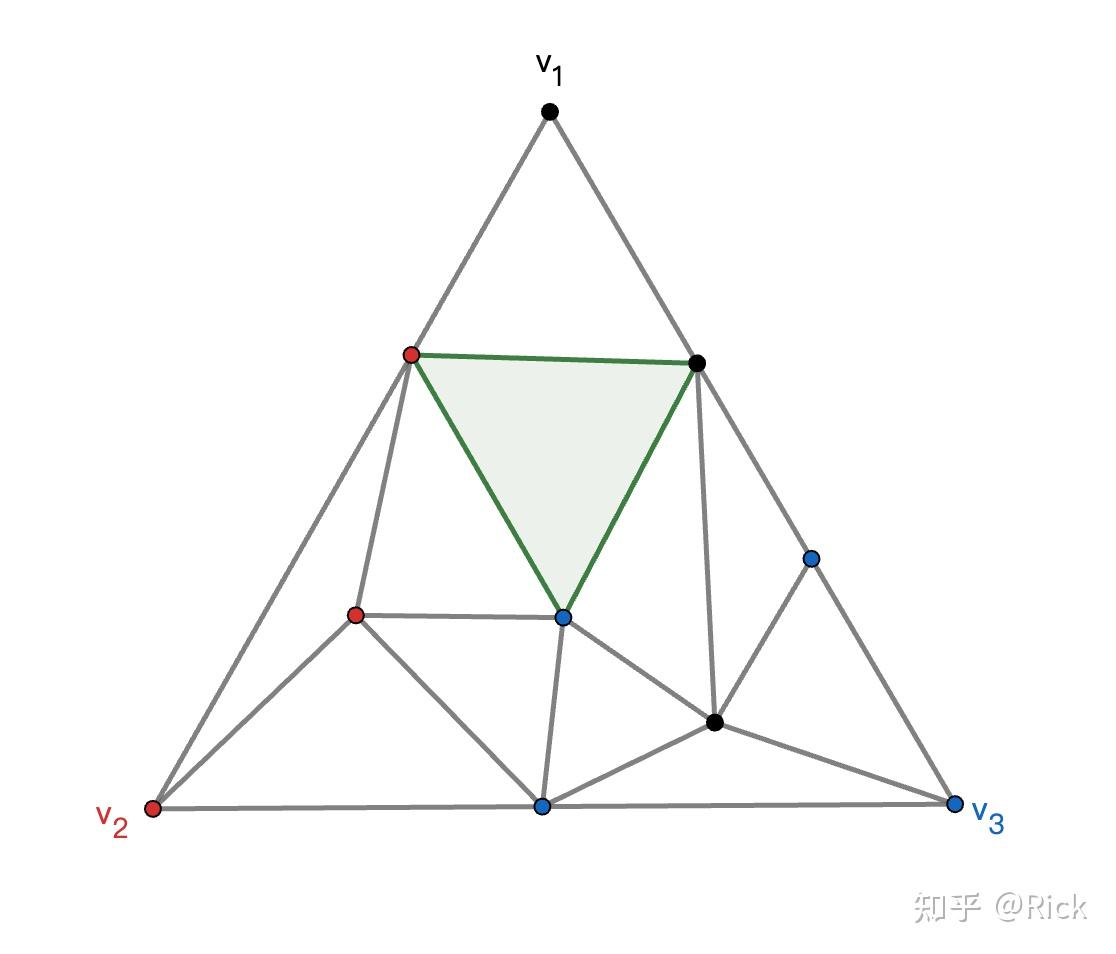
\includegraphics[scale=0.2]{Figures/SpernerLemma.jpg}
            \caption[SpernerLemma]{Sperner引理示意图}
        \end{figure}
    \end{lemma}

    它们一个是拓扑的定理, 一个是组合的定理, 看似没有联系, 但实际上我们能证明它们是等价的: 由于 $B^n\cong K$, 我们将 Brouwer不动点定理的叙述改为 $K$ 到自身的连续映射 $f$ 必有不动点.

    $1^{\circ}$:Sperner引理 $\Rightarrow$ Brouwer不动点定理
    
    设 $K = [v_0,\dots,v_n]$ 是 $n$ 维单形, 对 $\forall x\in K$, $x=\sum_i\alpha_iv_i,\,\alpha_i\geqslant0,\,\sum_i\alpha_i=1$. 设 $f(x) = \sum_i\beta_iv_i$, 定义染色映射 
    $\lambda(x)$ 为使得 $\alpha_i\geqslant\beta_i$ 且 $\alpha_i\neq0$ 的最小下标 $i$. 我们首先观察到在任意集合 $\{i_0,\dots,i_k\}\subseteq\{0,\dots,n\}$ 中, 
    对 $\forall x\in[v_{i_0},\dots,v_{i_k}]$, $x$ 的坐标 $\alpha$ 满足 $\alpha_i=0,\,i\notin\{i_0,\dots,i_k\}$, 因此 $\lambda(x)$ 只可能在 $\{i_0,\dots,i_k\}$ 中取值.

    固定染色 $\lambda$, 取重心重分 $K^0,K^1,\dots$, 则在每一个 $K^j$ 中 $\lambda$ 均满足引理条件, 于是存在异色单形 $\Delta^j=[u^j_0,\dots,u^j_n]$, 不妨设 $\lambda(u^j_i)=i$.
    因为 $K$ 是紧集, 因此 $\{u^j_0\}_j$ 存在收敛子列, 不妨设就为序列本身, 由重心重分的性质知 $\Delta^j$ 的直径趋于零, 因此对所有 $i$, $\{u^j_i\}_j$ 均收敛于同一点 $u$, 即 
    $u=\lim\limits_{j\rightarrow\infty}u^j_i,\,\forall\,i=0,\dots,n$. 由染色的定义知 $u^j_i$ 的 $v_i$ 坐标不等于零且大于等于 $f(u^j_i)$ 的, 
    根据极限的保号性知 $u$ 的所有坐标 $\alpha_i$ 大于等于 $f(u)$ 对应的坐标 $\beta_i$, 但因为 $\sum_i\alpha_i = \sum_i\beta_i = 1$, 所以 $\alpha_i=\beta_i$, 因此 $u = f(u)$ 是 $f$ 的不动点.

    $2^{\circ}$:Sperner引理 $\Leftarrow$ Brouwer不动点定理
    
    设 $K = [v_0,\dots,v_n]$ 是 $n$ 维单形, $\lambda$ 为满足引理要求的染色, $T$ 是 $K$ 的一个三角剖分, 则可以定义单纯映射 $f:K\rightarrow K$ 如下: 对 $\forall x\in V(T)$, 
    定义 $f(x) = v_{\lambda(x)}$, 若 $x = \sum_{i=0}^{k}\alpha_ix_i$, 其中 $[x_0,\dots,x_k]$ 为 $T$ 的 $k$ 维单形, 定义 $f(x) = \sum_{i=0}^{k}\alpha_iv_{\lambda(x_i)}$.

    若 $T$ 中没有 $n$ 维异色单形, 则 $f$ 的像集包含于 $\partial K$ 中, 且对于每个 $(n-1)$ 维面 $[v_0,\dots,\hat{v_i},\dots,v_n]$ 均有 $f([v_0,\dots,\hat{v_i},\dots,v_n])\subset[v_0,\dots,\hat{v_i},\dots,v_n]$.
    不妨设 $\sum_{i=0}^{n}v_i = 0$, 即 $K$ 的重心是原点. 定义 $g:\partial K\rightarrow \partial K$, $g(x)$ 为射线 $xO$ 与 $\partial K$ 的另一个交点, 类比对径映射. 则 $g([v_0,\dots,\hat{v_i},\dots,v_n])\cap[v_0,\dots,\hat{v_i},\dots,v_n]=\emptyset$
    则 $g\circ f$ 是 $K$ 到自身的连续映射, 但没有不动点, 与Brouwer不动点定理矛盾.

    现在我们回到Sperner引理本身的证明
    \begin{proof}
        对维数 $n$ 做归纳, 我们证明对任意维数异色单形的个数均为奇数.

        当 $n=1$ 时, $K = [v_0,v_1]$ 可看做闭区间 $[0,1]$, 设 $v_0=x_0<x_1<\cdots<x_m=v_1$ 是剖分 $T$ 中的点, 则 $\#\verb|异色单形| = \#\left\{i\,\big|\,\lambda(x_{i-1})\neq\lambda(x_i)\right\}$. 而
        \begin{equation*}
            1 = \lambda(v_1)-\lambda(v_0) = \sum_{i=1}^{m}\lambda(x_i)-\lambda(x_{i-1}) = \sum_{\lambda(x_{i-1})\neq\lambda(x_i)}\lambda(x_i)-\lambda(x_{i-1})
        \end{equation*} 
        因此 $\#\verb|异色单形|$ 是奇数. 

        假设维数为 $n-1$ 时命题成立, 我们称 $T$ 中的 $(n-1)$ 维单形 $[x_0,\dots,x_{n-1}]$ 为一个好单形, 若 $\{\lambda(x_0),\dots,\lambda(x_{n-1})\} = \{0,\dots,n-1\}$. 对 $T$ 中的  $n$ 维单形
        $\Delta_n=[u_0,\dots,u_n]$, 令 $c(\Delta_n)$ 为 $\Delta_n$ 中好单形的个数, 记 $S=\{\lambda(u_0),\dots,\lambda(u_n)\}$, 则
        \begin{equation*}
            c(\Delta_n)= \left\{
            \begin{aligned}
                0,\; &\{0,\dots,n-1\}\nsubseteq S \\
                2,\; &\{0,\dots,n-1\} = S \\
                1,\; &\{0,\dots,n\} = S  
            \end{aligned}\right. ,
        \end{equation*}
        于是异色单形个数的奇偶性与 $\sum\limits_{\Delta_n\subset T}c(\Delta_n)$ 的奇偶性相同. 而当好单形在 $\overset{\circ}{K}$ 内时, 它是两个 $n$ 单形的公共面; 当好单形在 $\partial K$ 上时, 它仅为一个 $n$ 单形的面.
        因此异色单形个数的奇偶性与 $\partial K$ 上好单形的个数的奇偶性相同, 根据条件好单形仅在 $[v_0,\dots,v_{n-1}]$ 中出现, 由归纳假设知 $[v_0,\dots,v_{n-1}]$ 中好单形有奇数个, 命题成立.
    \end{proof}

    \section{区域不变性定理(Invariance of domain)}
        该定理也是拓扑中的重要定理, 有人说它是欧式空间的内蕴性质, 用它可以区分不同维数的欧式空间.
        \begin{theorem}
            设 $U$ 为 $\mathbb{R}^n$ 中的开子集, $f:U\rightarrow\mathbb{R}^n$ 为连续单射, 则 $f(U)$ 为 $\mathbb{R}^n$ 的开子集且 $f$ 为开映射, 即 $f$ 为 $U$ 到 $f(U)$ 的同胚.
        \end{theorem} %引用代数拓扑章节
    % \chapter{图论与组合论}
    \section{图论}
    \subsection{一个关于二部图的小问题}
    \begin{problem}
        设有二部图 $(U,V)$, $U$ 的顶点数为 $12$, 且对任意 $U$ 的 $10$ 顶点子集 $X$, 集合 $\{v\,\big|\,v\verb|与某个|u\verb|相邻|,\;u\in X\}$ 大小为 $20$; 
        对任意 $U$ 的 $8$ 顶点子集 $Y$, 集合 $\{v\,\big|\,v\verb|与某个|u\verb|相邻|,\;u\in Y\}$ 大小为 $16$. 证明: 集合 $\{v\,\big|\,v\verb|与某个|u\verb|相邻|,\;u\in U\}$ 大小为 $24$.
    \end{problem}
    \begin{proof}
        对 $U$ 的任意子集 $X$, 记 $V_X = \{v\,\big|\,v\verb|与某个|u\verb|相邻|,\;u\in X\}$, 并记 $n(X) = |V_X|$, 特别地, 当 $X$ 仅有一个元素, 即 $X=\{u\}$ 时, $n(X)$ 写为 $n(u)={\rm deg}(u)$.
        继续记 $U_n$ 为 $U$ 的某个顶点数为 $n$ 的子集, 则题设可写为: 
        \begin{gather*}
            n(U_{10})=20,\quad\forall U_{10}\subset U \\
            n(U_8)=16,\quad\forall U_8\subset U
        \end{gather*}
        对 $U$ 的任意子集 $X,\,Y$, 
        \begin{align*}
            n(X\cup Y) &= |V_X\cup V_Y| = |V_X| + |V_Y| - |V_X\cap V_Y| \\
            &\leqslant |V_X| + |V_Y| - |V_{X\cap Y}| = n(X) + n(Y) - n(X\cap Y)
        \end{align*} 
        于是
        \begin{equation*}
            n(X) + n(Y) \geqslant n(X\cup Y) + n(X\cap Y)
        \end{equation*}
        我们将反复使用这个不等式推导出结论.

        对 $\forall\, U_6$, 存在 $U_8,U_8'$ 使得 $U_8\cap U_8'=U_6$, 则 $|U_8\cup U_8'| = 10$, 于是
        \begin{equation*}
            32 = n(U_8)+n(U_8') \geqslant n(U_8\cup U_8') + n(U_6) = 32 + n(U_6)
        \end{equation*}
        即 $n(U_6)\leqslant12$.

        对 $\forall\, U_4$, 存在 $U_6,U_6'$ 使得 $U_6\cap U_6'=U_4$, 则 $|U_6\cup U_6'| = 8$, 于是
        \begin{equation*}
            24 \geqslant n(U_6)+n(U_6') \geqslant n(U_6\cup U_6') + n(U_4) = 16 + n(U_4)
        \end{equation*}
        即 $n(U_4)\leqslant8$.

        对 $\forall\, U_2$, 存在 $U_4,U_6$ 使得 $U_4\cap U_6=U_2$, 则 $|U_4\cup U_6| = 6$, 于是
        \begin{equation*}
            20 \geqslant n(U_4)+n(U_6) \geqslant n(U_4\cup U_6) + n(U_2) = 16 + n(U_2)
        \end{equation*}
        即 $n(U_2)\leqslant4$. 

        另一方面对 $\forall\, U_2$, 存在 $U_8$ 使得 $U_2\cap U_8=\emptyset$, 则 $|U_2\cup U_8| = 10$, 于是
        \begin{equation*}
            16+n(U_2)=n(U_8)+n(U_2)\geqslant n(U_10)=20
        \end{equation*}
        即 $n(U_2)\geqslant4$. 于是 $n(U_2)=4$, 从而前面的不等式全为等式, 进而 $n(U_4) = 8$, $n(U_6) = 12$.
        对任意不相交的 $U_2,U_2'$, 
        \begin{equation*}
            8 = n(U_2\cup U_2') = n(U_2)+n(U_2')-|V_{U_2}\cap V_{U_2'}| = 8 - |V_{U_2}\cap V_{U_2'}|
        \end{equation*}
        推出 $|V_{U_2}\cap V_{U_2'}| = 0$, 也即 $V_{U_2}\cap V_{U_2'}=\emptyset$, 到此就能推出 $n(U) = 24$ 了.

        进一步研究二部图 $(U,V)$, 由上述不相交性质可知对任意不同两点 $u,u'$, $V_u\cap V_{u'}=\emptyset$, 于是 $n(u)+n(u') = n(\{u,u'\}) = 4$, 可推出所有的 $n(u) = 2$.
        设 $U = \{u_1,\dots,u_{12}\}$, 二部图的连接情况为 $E = \{(u_i,v_{2i-1}),\,(u_i,v_{2i})\}_{1\leqslant i\leqslant12}$. 
    \end{proof} %引用图论与组合论章节
    % \section{乘积与扩张}
    \begin{definition}[群的正合列]
        设有群 $N$、 $Q$, 则群 $Q$ 过群 $N$ 的扩张为如下群短正合列:
        \begin{center}
            \begin{tikzcd}
                1 \arrow[r] & N \arrow[r, "\iota"] & G \arrow[r, "\pi"] & Q \arrow[r] & 1
            \end{tikzcd}
        \end{center}
        也即 $\iota$ 是一个单同态, $\pi$ 是一个满同态, 且 ${\rm Im}\iota=\ker\pi$.
    \end{definition}

    扩张得到的群 $G$ 不一定能写成核与商群的直积, 比如下面介绍的半直积, 它给核一个 “扭转”.

    \begin{definition}[群的半直积]
        设有群 $N$、 $Q$, 且有同态 $\varphi:Q\rightarrow\Aut(N)$ (也即群 $Q$ 通过 $\varphi$ 作用于 $N$ 上).
        则群的半直积 $N\rtimes_{\varphi} Q$ 作为集合就是笛卡尔积 $N\times Q$, 其乘法定义为:
        \begin{align*}
            (N\rtimes_{\varphi}Q)\times(N\rtimes_{\varphi}Q)&\rightarrow(N\rtimes_{\varphi}Q) \\
            (n_1,q_1)\cdot(n_2,q_2)&\mapsto(n_1\cdot\varphi(q_1)(n_2),\,q_1\cdot q_2)
        \end{align*}
    \end{definition}
    \begin{remark}
        可以验证上述定义的乘法确实构成一个群:
        \begin{itemize}
            \item 结合律:
            \begin{align*}
                &\Big((n_1,q_1)\cdot(n_2,q_2)\Big)\cdot(n_3,q_3) \\
                =&\Big(n_1\cdot\varphi(q_1)(n_2),\,q_1q_2\Big)\cdot(n_3,q_3) \\
                =&\Big(n_1\cdot\varphi(q_1)(n_2)\cdot\varphi(q_2q_3)(n_3),\,(q_1q_2)q_3\Big) 
            \end{align*}
            \begin{align*}
                &(n_1,q_1)\cdot\Big((n_2,q_2)\cdot(n_3,q_3)\Big) \\
                =&(n_1,q_1)\cdot\Big(n_2\cdot\varphi(q_2)(n_3),\,q_2q_3\Big) \\
                =&\Big(n_1\cdot\varphi(q_1)(n_2\cdot\varphi(q_2)(n_3)),\,q_1(q_2q_3)\Big)
            \end{align*}
            而
            \begin{align*}
                &n_1\cdot\varphi(q_1)(n_2\cdot\varphi(q_2)(n_3)) \\
                =&n_1\cdot\varphi(q_1)(n_2)\cdot\varphi(q_1)\varphi(q_2)(n_3) \\
                =&n_1\cdot\varphi(q_1)(n_2)\cdot\varphi(q_2q_3)(n_3)
            \end{align*}
            因此上述乘法满足结合律.
            \item 我们也可以算一下在这个乘法下的逆:
            \begin{gather*}
                (n_1,q_1)\cdot(n_2,q_2) = \Big(n_1\cdot\varphi(q_1)(n_2),\,q_1q_2\Big) = (e_N,e_Q) \\
                \Rightarrow q_2 = q_1^{-1},\quad n_2 = \varphi(q_1^{-1})(n_1^{-1})
            \end{gather*}
        \end{itemize}

        \begin{definition}[分裂的正合列]
            我们称一个正合列
            \begin{center}
                \begin{tikzcd}
                    1 \arrow[r] & N \arrow[r, "\iota"] & G \arrow[r, "\pi"] & Q \arrow[r] & 1
                \end{tikzcd}
            \end{center}
            分裂, 若存在群同态 $s:Q\rightarrow G$ 使得 $\pi\circ s=\id_Q$. 也即 $Q$ 能嵌入 $G$ 中.
        \end{definition}
        \begin{remark}[群的半直积与分裂的正合列]
            若有同态 $\varphi:Q\rightarrow\Aut(N)$, 则短正合列
            \begin{center}
                \begin{tikzcd}
                    1 \arrow[r] & N \arrow[r, "\iota"] & N\rtimes_{\varphi}Q \arrow[r, "\pi"] & Q \arrow[r] & 1
                \end{tikzcd}
            \end{center}
            是分裂的. 
            
            这里 $\iota:N\rightarrow N\rtimes_{\varphi}Q$ 是嵌入到第一个分量给出的同态, $\pi:N\rtimes_{\varphi}Q\rightarrow Q$ 是投射到第二个分量给出的同态.
            分裂映射由
            \begin{align*}
                Q &\rightarrow N\rtimes_{\varphi}Q \\
                q &\mapsto(e,q)
            \end{align*}
            给出.

            反过来, 在一个分裂的群扩张中, 扩张得到的群可以写成核与商群的半直积: 设有分裂的正合列
            \begin{center}
                \begin{tikzcd}
                    1 \arrow[r] & N \arrow[r, "\iota"] & G \arrow[r, "\pi",shift left=0.3ex, harpoon] & Q \arrow[r] \arrow[l, "s",shift left=0.3ex, harpoon] & 1
                \end{tikzcd}
            \end{center}
            则可以定义映射
            \begin{align*}
                N\rtimes_{\varphi}Q&\rightleftharpoons G \\
                (n,q)&\mapsto n\cdot s(q) \\
                \Big(g\cdot(s\circ\pi(g))^{-1},\,\pi(g)\Big)&\reflectbox{$\mapsto$}\,g
            \end{align*}
            可以验证它们是互逆的群同态, 其中 $Q$ 在 $N$ 上的作用为
            \begin{align*}
                \varphi: Q & \rightarrow\Aut(N) \\
                q & \mapsto\big(n\mapsto s(q)\cdot n\cdot s(q)^{-1}\big).
            \end{align*}
        \end{remark}
        
        让我们仔细解释一下每个映射的由来, 在分裂的群扩张中, $N$ 和 $Q$ 均可视作 $G$ 的一个子群, 从 $N\rtimes_{\varphi}Q$ 到 $G$ 的映射就是将两个分量重新组合到一起的过程;
        从 $G$ 到 $N\rtimes_{\varphi}Q$ 的映射就是将两个分量提取出来的过程. 为了保证映射是群同态, 我们需要 $N\rtimes_{\varphi}Q$ 满足特定的乘法, 也就是说我们需要特定的群作用 
        $Q\overset{\varphi}{\curvearrowright}N$. 群同态要求:
        \begin{align*}
            n_1\cdot s(q_1)\cdot n_2\cdot s(q_2)&=n_1\cdot \varphi(q_1)(n_2)\cdot s(q_1q_2) \\
            \varphi(q_1)(n_2)&=s(q_1)\cdot n_2\cdot s(q_1)^{-1}
        \end{align*}
        因此 $\varphi$ 只能形如共轭作用, 这也解释了半直积比直积多出来的“扭转”. 注意到若 $N$ 和 $Q$ 中的元素可交换, 群作用平凡, 此时 $Q$ 自动成为 $G$ 的正规子群, 且 $N\rtimes_{\varphi}Q = N\times Q$.
    \end{remark} %引用群论章节

    \part{杂题集萃}
    % \chapter{组合论}
    \section{图论}
    \subsection{一个关于二部图的小问题}
    \begin{problem}
        设有二部图 $(U,V)$, $U$ 的顶点数为 $12$, 且对任意 $U$ 的 $10$ 顶点子集 $X$, 集合 $\{v\,\big|\,v\verb|与某个|u\verb|相邻|,\;u\in X\}$ 大小为 $20$; 
        对任意 $U$ 的 $8$ 顶点子集 $Y$, 集合 $\{v\,\big|\,v\verb|与某个|u\verb|相邻|,\;u\in Y\}$ 大小为 $16$. 证明: 集合 $\{v\,\big|\,v\verb|与某个|u\verb|相邻|,\;u\in U\}$ 大小为 $24$.
    \end{problem}
    \begin{proof}
        对 $U$ 的任意子集 $X$, 记 $V_X = \{v\,\big|\,v\verb|与某个|u\verb|相邻|,\;u\in X\}$, 并记 $n(X) = |V_X|$, 特别地, 当 $X$ 仅有一个元素, 即 $X=\{u\}$ 时, $n(X)$ 写为 $n(u)={\rm deg}(u)$.
        继续记 $U_n$ 为 $U$ 的某个顶点数为 $n$ 的子集, 则题设可写为: 
        \begin{gather*}
            n(U_{10})=20,\quad\forall U_{10}\subset U \\
            n(U_8)=16,\quad\forall U_8\subset U
        \end{gather*}
        对 $U$ 的任意子集 $X,\,Y$, 
        \begin{align*}
            n(X\cup Y) &= |V_X\cup V_Y| = |V_X| + |V_Y| - |V_X\cap V_Y| \\
            &\leqslant |V_X| + |V_Y| - |V_{X\cap Y}| = n(X) + n(Y) - n(X\cap Y)
        \end{align*} 
        于是
        \begin{equation*}
            n(X) + n(Y) \geqslant n(X\cup Y) + n(X\cap Y)
        \end{equation*}
        我们将反复使用这个不等式推导出结论.

        对 $\forall\, U_6$, 存在 $U_8,U_8'$ 使得 $U_8\cap U_8'=U_6$, 则 $|U_8\cup U_8'| = 10$, 于是
        \begin{equation*}
            32 = n(U_8)+n(U_8') \geqslant n(U_8\cup U_8') + n(U_6) = 32 + n(U_6)
        \end{equation*}
        即 $n(U_6)\leqslant12$.

        对 $\forall\, U_4$, 存在 $U_6,U_6'$ 使得 $U_6\cap U_6'=U_4$, 则 $|U_6\cup U_6'| = 8$, 于是
        \begin{equation*}
            24 \geqslant n(U_6)+n(U_6') \geqslant n(U_6\cup U_6') + n(U_4) = 16 + n(U_4)
        \end{equation*}
        即 $n(U_4)\leqslant8$.

        对 $\forall\, U_2$, 存在 $U_4,U_6$ 使得 $U_4\cap U_6=U_2$, 则 $|U_4\cup U_6| = 6$, 于是
        \begin{equation*}
            20 \geqslant n(U_4)+n(U_6) \geqslant n(U_4\cup U_6) + n(U_2) = 16 + n(U_2)
        \end{equation*}
        即 $n(U_2)\leqslant4$. 

        另一方面对 $\forall\, U_2$, 存在 $U_8$ 使得 $U_2\cap U_8=\emptyset$, 则 $|U_2\cup U_8| = 10$, 于是
        \begin{equation*}
            16+n(U_2)=n(U_8)+n(U_2)\geqslant n(U_10)=20
        \end{equation*}
        即 $n(U_2)\geqslant4$. 于是 $n(U_2)=4$, 从而前面的不等式全为等式, 进而 $n(U_4) = 8$, $n(U_6) = 12$.
        对任意不相交的 $U_2,U_2'$, 
        \begin{equation*}
            8 = n(U_2\cup U_2') = n(U_2)+n(U_2')-|V_{U_2}\cap V_{U_2'}| = 8 - |V_{U_2}\cap V_{U_2'}|
        \end{equation*}
        推出 $|V_{U_2}\cap V_{U_2'}| = 0$, 也即 $V_{U_2}\cap V_{U_2'}=\emptyset$, 到此就能推出 $n(U) = 24$ 了.

        进一步研究二部图 $(U,V)$, 由上述不相交性质可知对任意不同两点 $u,u'$, $V_u\cap V_{u'}=\emptyset$, 于是 $n(u)+n(u') = n(\{u,u'\}) = 4$, 可推出所有的 $n(u) = 2$.
        设 $U = \{u_1,\dots,u_{12}\}$, 二部图的连接情况为 $E = \{(u_i,v_{2i-1}),\,(u_i,v_{2i})\}_{1\leqslant i\leqslant12}$. 
    \end{proof} %引用组合问题
    % \chapter{高等代数}
    \begin{problem}
        假设 $n$ 维欧氏空间 $V$ 中有 $m$ 个向量两两成钝角, 证明: $m\leqslant n+1$.
    \end{problem}

    \begin{proof}
        当 $\mathrm{dim}V = 1$, 命题显然成立.

        假设当维数为 $n-1$ 时命题成立, 现证明命题在 $n$ 维时仍成立. 设 $\ft{v}{1}{m}$ 为 $V$ 中两两成钝角的向量, 
        令 $W$ 为 $Lv_m$ 的正交补空间, 并记 $P:V\rightarrow W$ 为正交投影映射, 令 $w_1=Pv_1,\dots,w_{m-1}=Pv_{m-1}$, 则当 $i\neq j$ 时, 
        \begin{align*}
            <w_i, w_j> &= <Pv_i,Pv_j> = \left<v_i-\frac{<v_i,v_m>}{<v_m,v_m>}v_m, v_j-\frac{<v_j,v_m>}{<v_m,v_m>}v_m\right> \\
            &=<v_i,v_j> - \frac{<v_i,v_m>\cdot<v_j,v_m>}{<v_m,v_m>} \\
            &<0
        \end{align*}
        因此 $\ft{w}{1}{m-1}$ 是 $n-1$ 维空间 $W$ 中两两成钝角的向量, 由归纳假设知 $m-1\leqslant n$, 即 $m\leqslant n+1$.
    \end{proof}
    \begin{remark}
        我感觉这和 $n$ 维欧氏空间的拓扑性质有关系, 
    \end{remark} %引用代数问题
    % \chapter{纤维丛}
    \begin{problem}
        Show that the fiber bundle
        \begin{center}
            \begin{tikzcd}
                S^3 \arrow[r] & S^{4n+3} \arrow[d] \\
                              & \mathbb{H}P^n                    
            \end{tikzcd}
        \end{center}
        gives rise to a quotient fiber bundle 
        \begin{center}
            \begin{tikzcd}
                S^2 \arrow[r] & \mathbb{C}P^{2n+1} \arrow[d] \\
                              & \mathbb{H}P^n                   
            \end{tikzcd}
        \end{center}
        by factoring out the action of $S^1$ on $S^{4n+3}$ by complex scalar multyplication.
    \end{problem}
    \begin{proof}
        Identifying quaternionic $n$-space $\mathbb{H}^n$ with complex $2n$-space $\mathbb{C}^{2n}$ in the standard way. 
        We get an identifycation of the unit spheres
        \begin{equation*}
            S^{4n-1}\cong S(\mathbb{C}^{2n})\cong S(\mathbb{H}^n),
        \end{equation*}
        especially we have
        \begin{equation*}
            S^3\cong S(\mathbb{C}^2)\cong S(\mathbb{H}).
        \end{equation*}

        By definition, $\mathbb{H}P^n$ is the orbit manifold of $\mathbb{H}^*$ acting on $(\mathbb{H}^{n+1})^*$ by scalar multyplication.
        后面的很好看出来。
    \end{proof} %引用拓扑问题
    % \chapter{尺规作图}
\begin{problem}[怀新一题 | 双曲测地线]
    给定欧几里得平面上的一个圆 $C_1$ 和两个不同的点 $A$,$B$。假设过 $A$,$B$ 的直线不经过 $C_1$ 的圆心。
    用直尺(没有刻度)和圆规作出一个过 $A$,$B$ 的圆 $C_2$,使得 $C_1$ 和 $C_2$交于两个点 $P$,$Q$,并且在交点 $P$,$Q$ 处垂直。
    注意 $A$,$B$ 分别可以在 $C_1$ 内,$C_1$ 外或 $C_1$ 上。
\end{problem}
\begin{proof}
    分析题目, 我们知道双曲平面有几种经典模型, 其中两种是 Poicar\'e 圆盘模型和上半平面模型. 在圆盘模型中, 过单位圆内两点的测地线经过延长后与边界正交, 所以要么是直径,
    要么就是题目所求的圆 $C_2$ 的一部分.
    \begin{figure}[htbp]
        \centering
        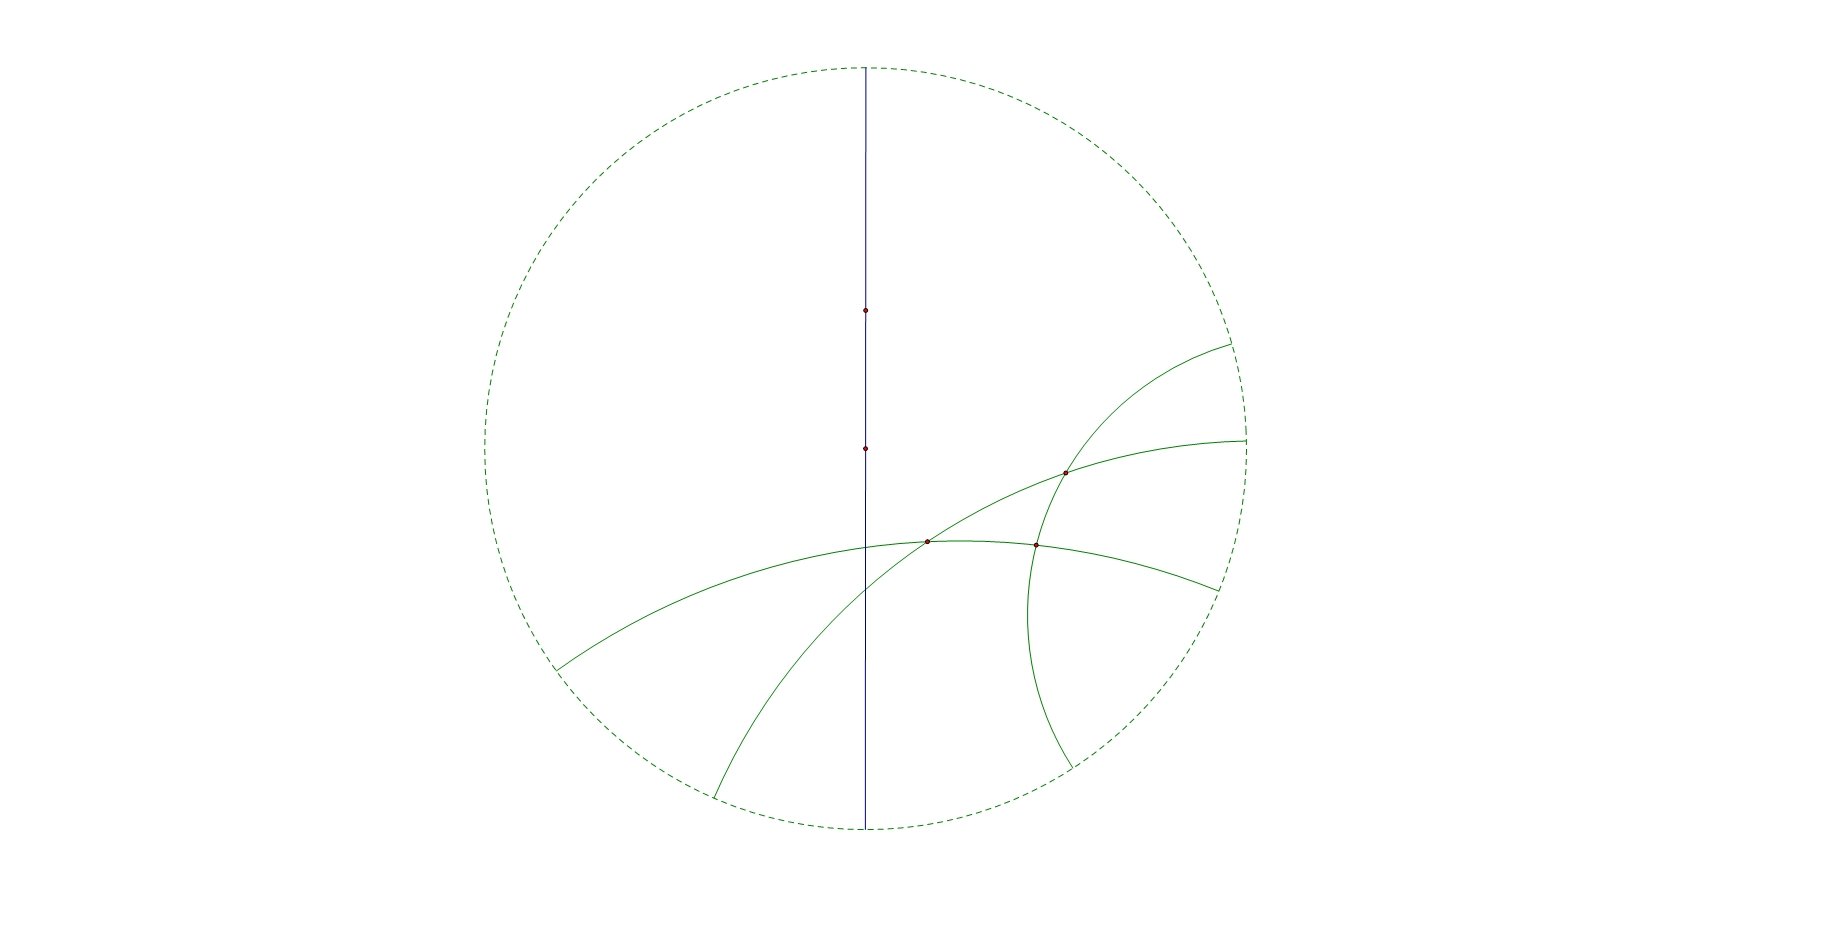
\includegraphics[scale = 0.18]{Figures/geo-in-D2.png}
        \caption{Poincar\'e 圆盘模型中的测地线}
    \end{figure}

    在上半平面模型中过两点的测地线经延长后要么是与横轴垂直的射线, 要么是与横轴正交的上半圆. 
    \begin{figure}[htbp]
        \centering
        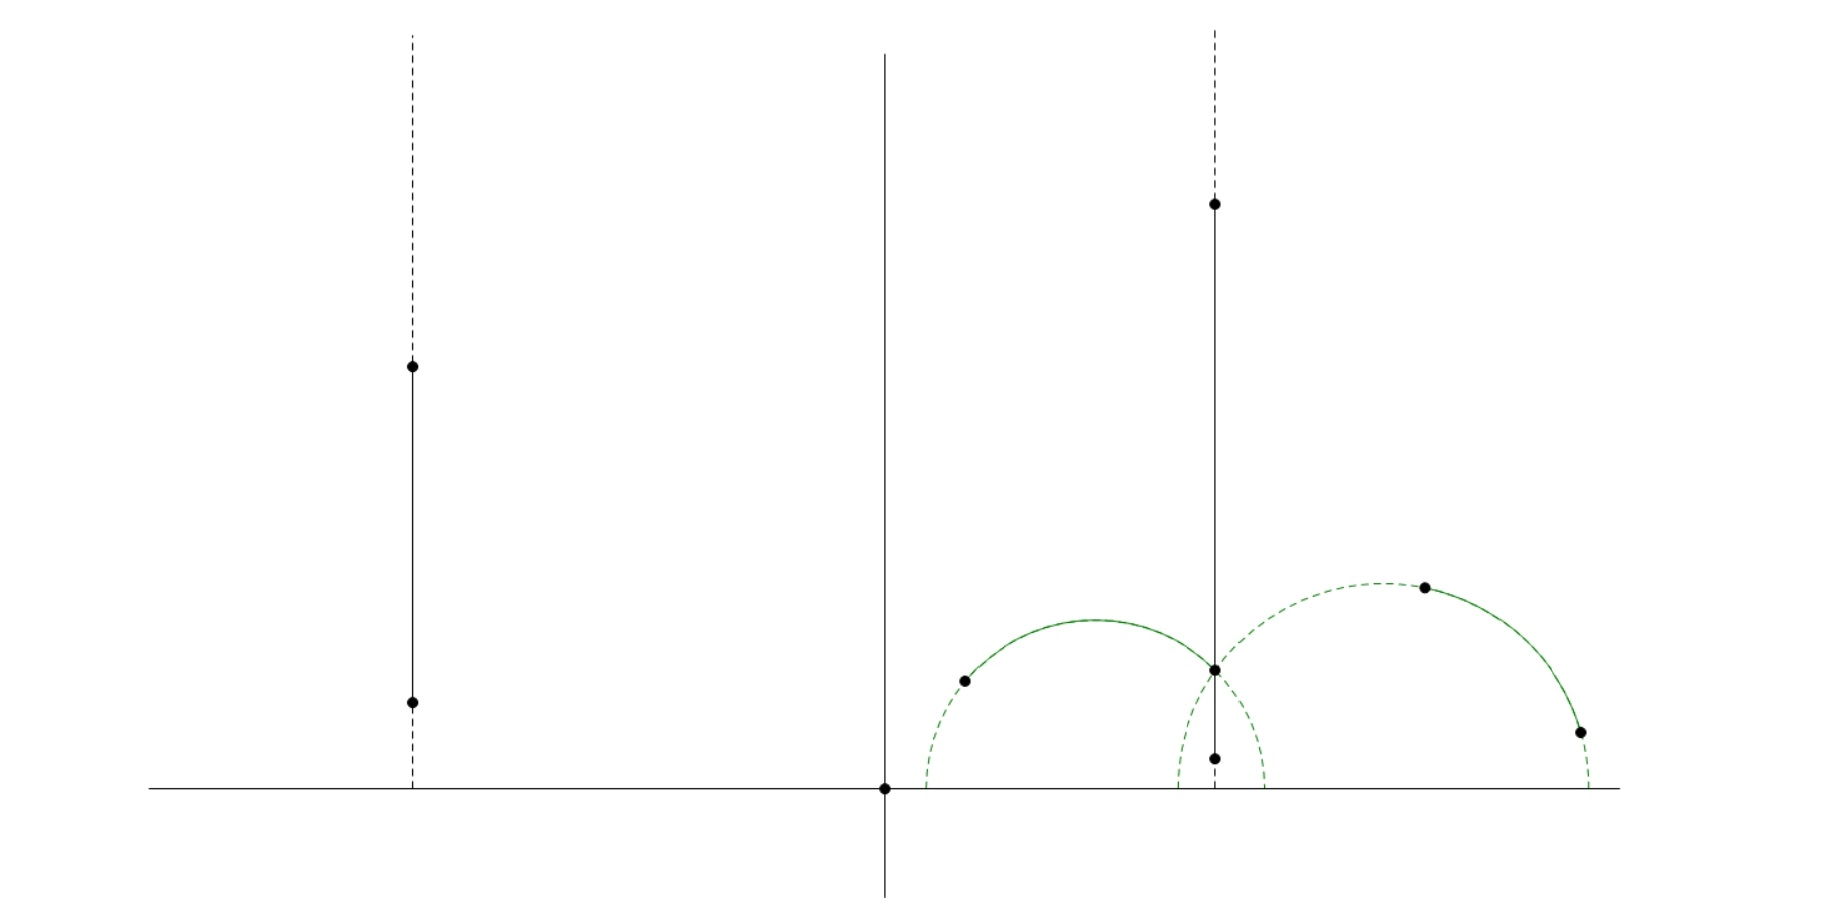
\includegraphics[scale = 0.2]{Figures/geo-in-H2.png}
        \caption{上半平面模型中的测地线}
    \end{figure}

    同时两个模型之间也有相互转化的关系, 用坐标表达就是 Cayley 变换, 用平面几何的语言就是反演变换. 于是我们可以用反演变换将原问题转化为:

    给定一条直线 $l$ 以及两点 $A'$, $B'$. 假设过 $A'$, $B'$ 的直线不与 $l$ 垂直, 用尺规作出一个过 $A'$,$B'$ 的圆 $C_2'$, 使得 $l$ 和 $C_2$交于两个点 $P'$,$Q'$, 并且在交点 $P'$,$Q'$ 处垂直. 
    
    注意到最后一个垂直条件实际上等价于圆心 $C_2'$ 在直线 $l$ 上, 于是我们把原来复杂的问题转化为一个简单的尺规作图问题.

    下面开始陈述作图过程, 简便起见我们略去一些基础尺规作图的过程.
    \begin{enumerate}
        \item 在圆 $C_1$ 上任取一点 $X$, 以 $D$ 为圆心作圆 $X$ 使其与圆 $C_1$ 交于两点 $E$, $F$. 连接 $E$, $F$ 得到直线 $l$, 此即圆 $C_1$ 关于圆 $D$ 反演后的图形.
        \item 连接线段 $DA$, 取其中点 $M$, 以 $M$ 为圆心, $MD$ 为半径作圆 $M$. 设圆 $M$ 交圆 $D$ 于两点 $G$, $H$, 连接线段 $GH$ 交线段 $AD$ 于点 $A'$, 此即点 $A$ 关于圆 $D$ 反演后的图形. 
        \item 同理可作点 $B$ 关于圆 $D$ 反演后的点 $B'$.
        \item 作线段 $A'B'$ 的中垂线, 交直线 $l$ 于点 $C_2'$, 由题目条件可知 $A'B'$ 不可能与 $l$ 垂直, 因此交点 $C_2'$ 一定存在.
        \item 类似地作出 $C_2'$ 关于圆 $D$ 反演后的点 $C_2$, 以 $C_2$ 为圆心, $CA$ 为半径作圆, 此即所求.
    \end{enumerate}
    \begin{figure}[htbp]
        \centering
        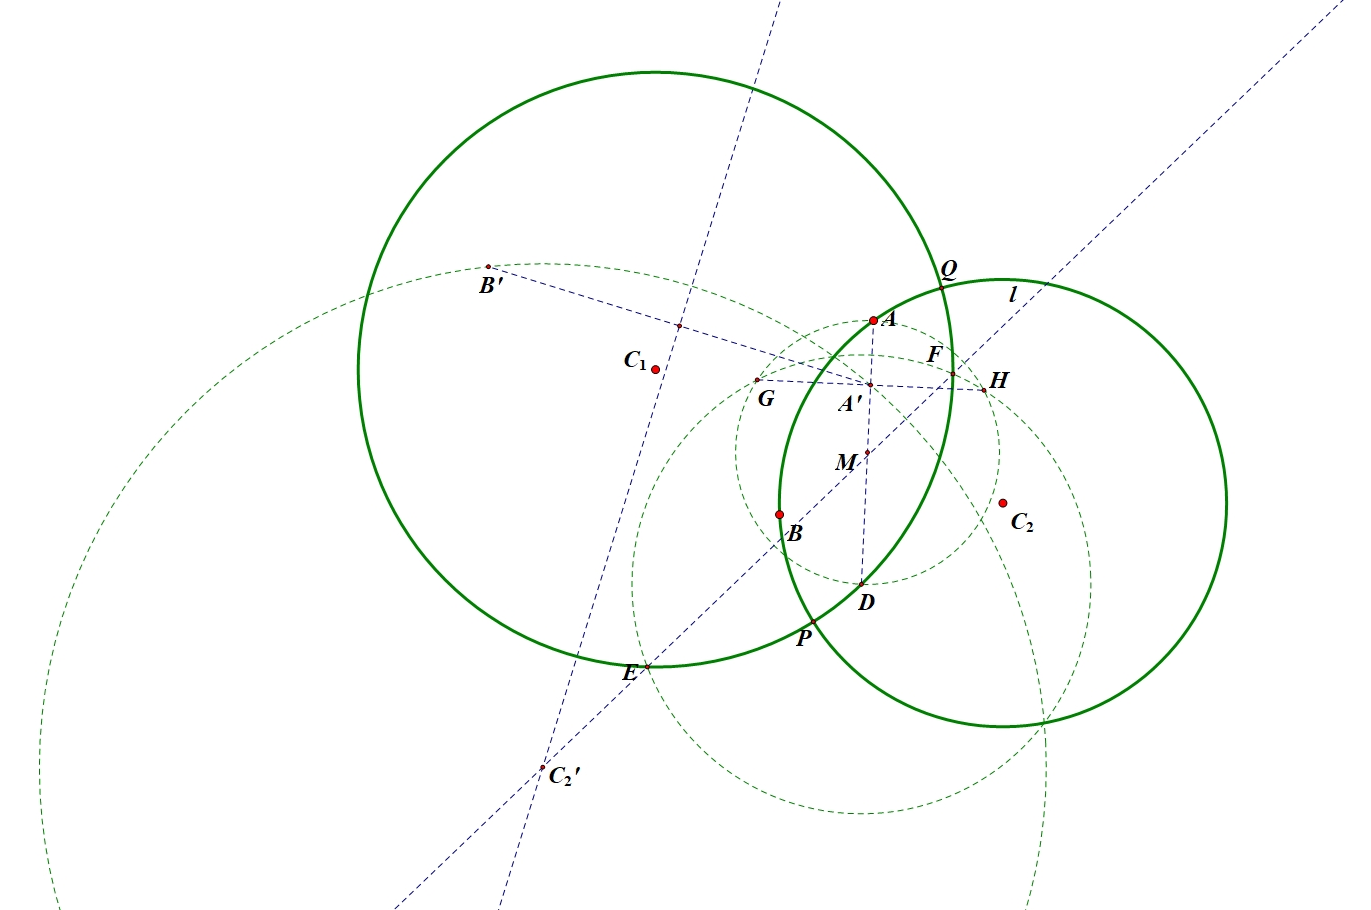
\includegraphics[scale = 0.4]{Figures/怀新一题(1).png}
    \end{figure}
\end{proof}
\begin{remark}
    此做法与点 $A$, $B$ 和圆 $C_1$ 的位置关系无关, 例如下面几种位置关系:
    \begin{figure}[htbp]
        \centering
        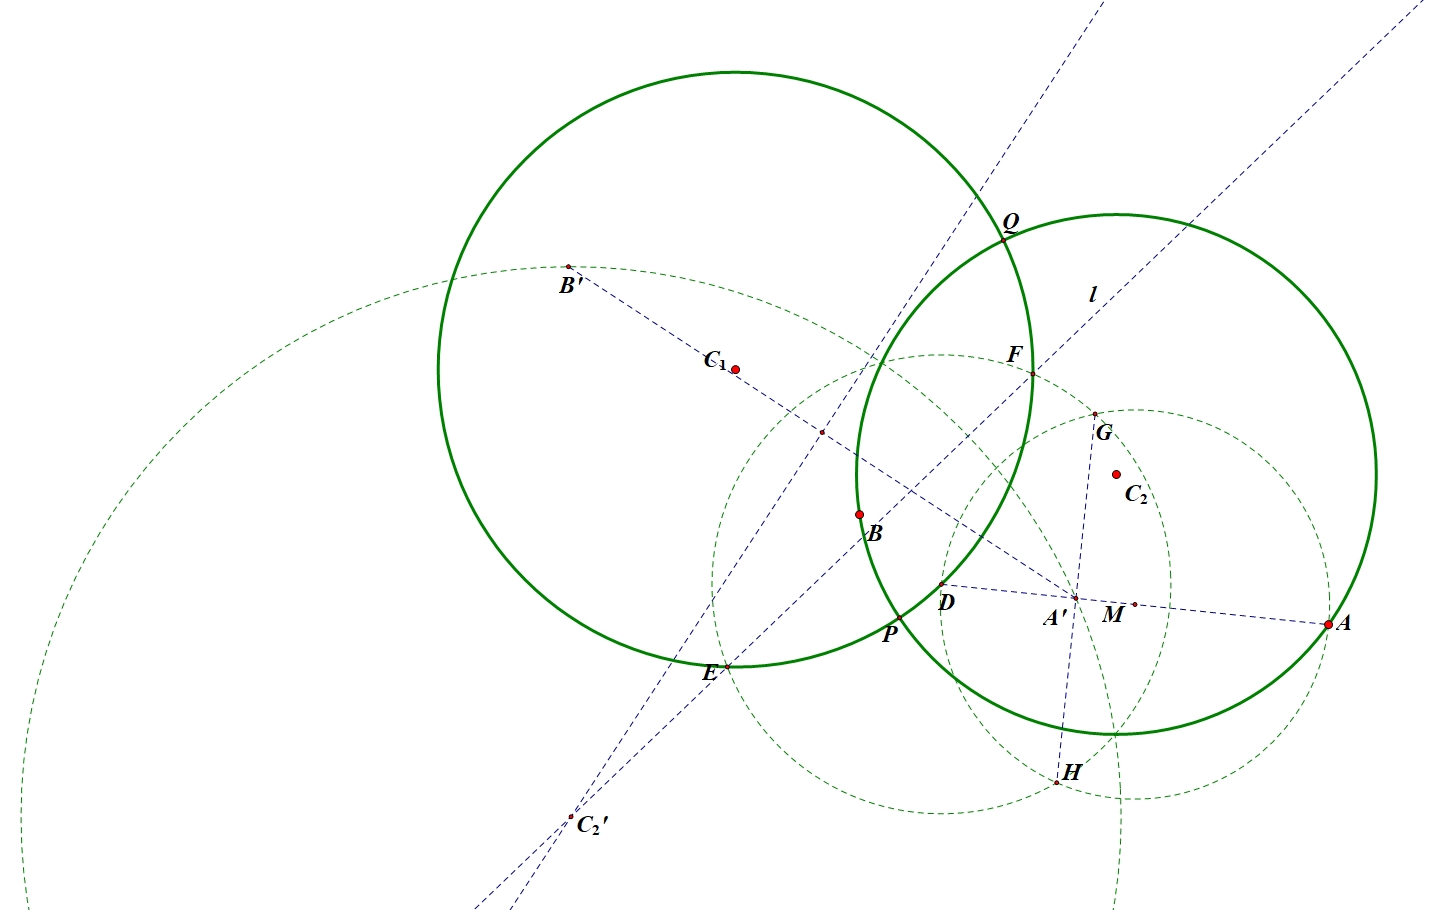
\includegraphics[scale = 0.31]{Figures/怀新一题(2).png}
        \caption{点 $A$ 在圆外, 点 $B$ 在圆内}                 
    \end{figure}
    \begin{figure}[htbp]
        \centering
        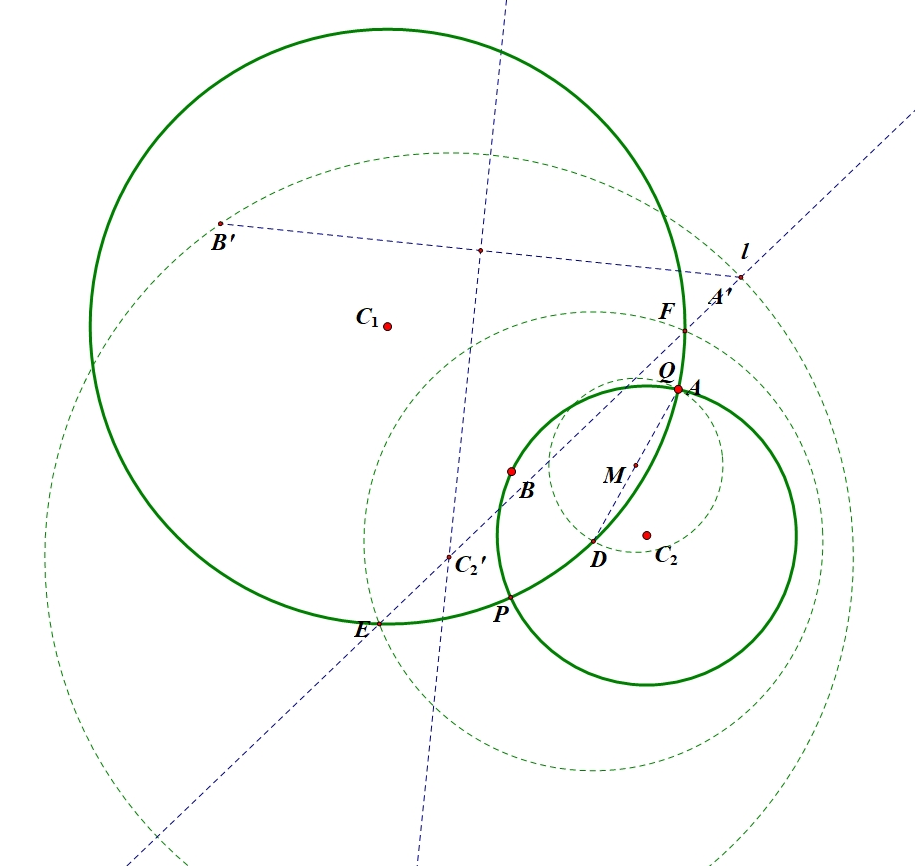
\includegraphics[scale = 0.31]{Figures/怀新一题(3).png}
        \caption{点 $A$ 在圆上, 点 $B$ 在圆内}
    \end{figure}
    \begin{figure}[htbp]
        \centering            
        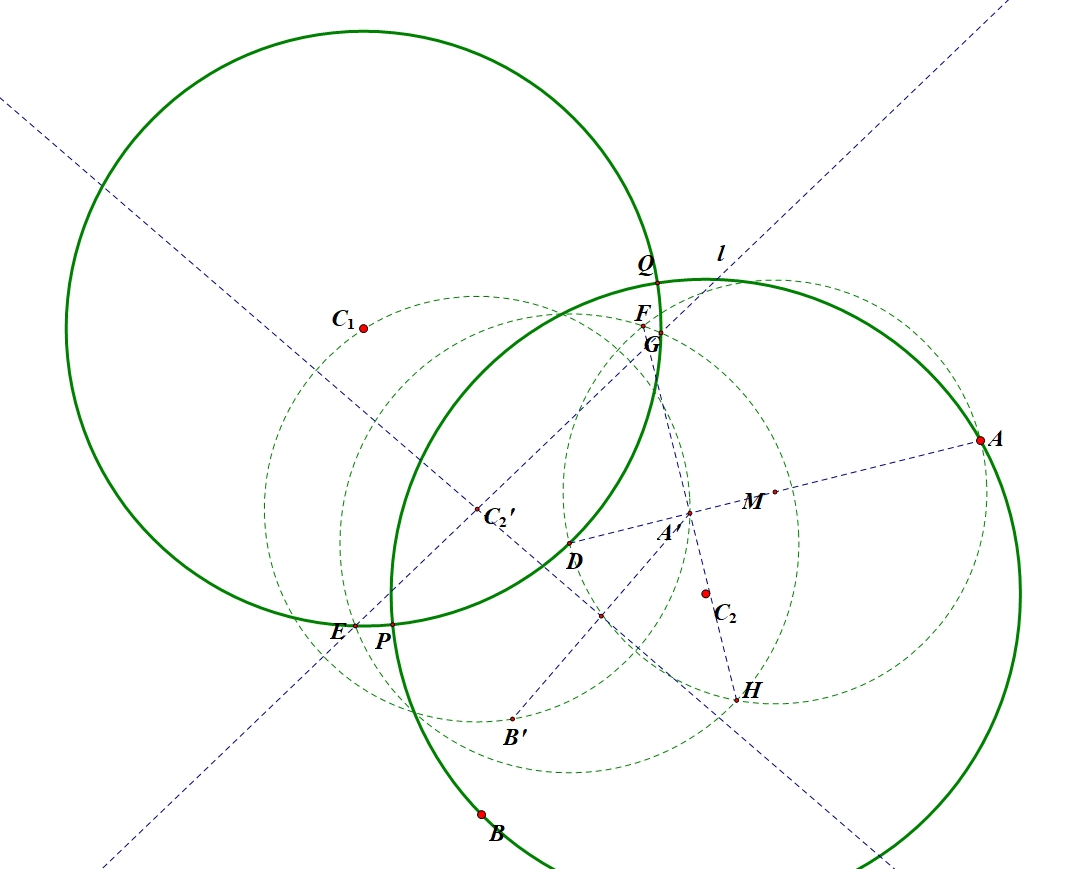
\includegraphics[scale = 0.31]{Figures/怀新一题(4).png}
        \caption{点 $A$, $B$ 均在圆外}
    \end{figure}
\end{remark} %引用几何问题

    \part{易错知识} %收录各种例子与反例,收录各种易错的小细节
    % \chapter{\Lie 群}
    \section{\Lie 群的连通性和单连通性在重要定理中的作用}
        开始前我们先叙述 \Lie 群中的一个重要定理:
        \begin{theorem}[\Lie 代数同态提升为 \Lie 群同态]\label{thm:Lifting-LieAlgebraHom-to-LieGroupHom}
            设 $G,H$ 是 \Lie 群, $G$ 既连通又单连通, $\mathfrak{g},\mathfrak{h}$ 分别是 $G,H$ 的 \Lie 代数.
            若 $\rho:\mathfrak{g}\rightarrow\mathfrak{h}$ 是一个 \Lie 代数同态, 则存在唯一的 \Lie 群同态 $\Phi:G\rightarrow H$ 
            满足 $\md\Phi = \rho$.
        \end{theorem}
        需要注意定理中 $G$ 的单连通和连通的条件缺一不可.
        \begin{example}
            若 $G$ 不是单连通的, 则这样的 $\Phi$ 不一定存在.

            \Lie 群 $(S^1,\cdot)$ 和 $(\mR,+)$ 的 \Lie 代数均为 $\mR$, 但不存在 $S^1$ 到 $\mR$ 的非平凡 \Lie 群同态. 
            设 $\varphi:S^1\rightarrow\mR$ 为 \Lie 群同态, 取 $S^1$ 的一个稠密子群 $\me^{i\pi\mQ}:=\left\{\me^{i\pi\theta}\,\big|\,\theta\in\mQ\right\}$, 
            则因为 $\me^{i\pi\mQ}$ 中的元素都是有限阶的, $\varphi(\me^{i\pi\mQ}) = \{0\}$. 由 $\varphi$ 的连续性可得 $\varphi(S^1) = \{0\}$. 因此 $\varphi$ 只能是平凡群同态.
        \end{example}
        \begin{example}
            若 $G$ 不是连通的, 则就算每个连通分支都是单连通的也不一定存在这样的 $\Phi$.

            考虑 $\mR\rtimes\mZ_2$, $\mZ_2$ 在 $\mR$ 上的作用由 $0\rightarrow\id,\,1\rightarrow-\id$ 给出. $\mR\rtimes\mZ_2$ 和 $\mR$ 的 \Lie 代数均为 $\mR$, 
            但 $\mR$ 到自身的恒同映射无法提升为 $\mR\rtimes\mZ_2$ 到 $\mR$ 的同态.

            假设这样的同态 $\varphi$ 存在, 取 $\mR\rtimes\mZ_2$ 包含 $(0,0)$ 的分支, 它是连通且单连通的 \Lie 群, 因此由定理{\rm\ref{thm:Lifting-LieAlgebraHom-to-LieGroupHom}}的唯一性知
            \begin{align*}
                \varphi:\mR\times\{0\}&\rightarrow\mR \\
                (t,0)&\mapsto t,\quad\forall\,t\in\mR
            \end{align*}
            又因为 $(0,1)$ 是 $\mR\rtimes\mZ_2$ 的 $2$ 阶元, 因此 
            \begin{equation*}
                \varphi:(0,1)\mapsto 0
            \end{equation*}
            但是
            \begin{equation*}
                \varphi\Big((0,1)\cdot(t,0)\Big) = \varphi(-t,0) = -t \neq 0+t = \varphi(0,1)+\varphi(t,0),\quad t\neq0.
            \end{equation*}
            因此这样的群同态 $\varphi$ 不可能存在.
        \end{example} %引用李群易错知识点
    % \chapter{复几何}

    \begin{example}
        设 $h(\cdot,\cdot)$ 是全纯向量丛 $E$ 的 ${\rm Hermitian}$ 度量, $D$ 为联络, $s,\,t$ 为 $E$ 的光滑截面, $\xi$ 是全纯切向量场. 则:
        \begin{itemize}
            \item $h(Ds,t)(\xi) = h(Ds(\xi),t)=h(D_{\xi}s,t)$
            \item $h(s,Dt)(\xi) = h(s,Dt(\textcolor{red}{\bar{\xi}}))=h(s,D_{\textcolor{red}{\bar{\xi}}}t)$ 
        \end{itemize}
        问题的关键是 ${\rm Hermitian}$ 度量关于第一个分量线性而关于第二个分量共轭线性.
    \end{example} %引用复几何易错知识点
\end{document}

